\documentclass[12pt,a4paper]{report}
\usepackage{fontspec}
\setmainfont{TeX Gyre Termes}
\setmonofont{TeX Gyre Cursor}
\usepackage[top=2.5cm,bottom=2.5cm,left=3.2cm,right=2cm]{geometry}
\usepackage{setspace}\setstretch{1.3}
\usepackage{indentfirst}\setlength{\parindent}{1cm}\setlength{\parskip}{3pt}
\usepackage{graphicx,float,longtable,array,colortbl,xcolor,booktabs}
\usepackage{enumitem}\setlist{itemsep=2pt,topsep=3pt}
\usepackage{titlesec}
\titleformat{\chapter}[display]{\centering\bfseries\Large}{\MakeUppercase{\chaptername}\ \thechapter}{8pt}{\Large\MakeUppercase}
\titlespacing*{\chapter}{0pt}{-10pt}{22pt}
\titleformat{\section}{\bfseries\large}{\thesection.}{0.6em}{}
\titleformat{\subsection}{\bfseries\normalsize}{\thesubsection.}{0.6em}{}
\usepackage{caption}
\captionsetup{font=small,labelfont=bf,labelsep=period}
\captionsetup[table]{position=top}
\usepackage{fvextra}
\fvset{fontsize=\footnotesize,breaklines=true,breakanywhere=true,frame=single,framesep=3pt,baselinestretch=1}
\PassOptionsToPackage{hyphens}{url}
\usepackage[hidelinks,unicode]{hyperref}
\urlstyle{same}\Urlmuskip=0mu plus 1mu
\usepackage{fancyhdr}
\pagestyle{fancy}\fancyhf{}\fancyhead[L]{\small Báo cáo đồ án cuối kỳ -- Lập trình Windows}
\fancyhead[R]{\small Quản lý mượn trả thiết bị}\fancyfoot[C]{\thepage}
\renewcommand{\headrulewidth}{0.4pt}
\fancypagestyle{plain}{\fancyhf{}\fancyfoot[C]{\thepage}\renewcommand{\headrulewidth}{0pt}}
\renewcommand{\chaptername}{Chương}
\renewcommand{\contentsname}{MỤC LỤC}
\renewcommand{\listtablename}{DANH MỤC BẢNG BIỂU}
\renewcommand{\listfigurename}{DANH MỤC HÌNH ẢNH}
\renewcommand{\tablename}{Bảng}
\renewcommand{\figurename}{Hình}
\renewcommand{\bibname}{TÀI LIỆU THAM KHẢO}
\renewcommand{\appendixname}{Phụ lục}
\counterwithin{table}{chapter}\counterwithin{figure}{chapter}
\newcommand{\code}[1]{\texttt{#1}}
\newcommand{\hinhphu}[2]{\begin{figure}[H]\centering
 \fbox{\parbox[c][5.2cm][c]{0.88\linewidth}{\centering\small\textbf{[ CHỪA CHỖ CHÈN ẢNH CHỤP MÀN HÌNH THỰC TẾ ]}\\[4pt] #2}}
 \caption{#1}\end{figure}}
\newcommand{\hinhanh}[3]{\IfFileExists{images/#1.png}{\begin{figure}[H]\centering\includegraphics[width=0.92\linewidth,height=0.45\textheight,keepaspectratio]{images/#1.png}\caption{#2}\end{figure}}{\IfFileExists{images/#1.jpg}{\begin{figure}[H]\centering\includegraphics[width=0.92\linewidth,height=0.45\textheight,keepaspectratio]{images/#1.jpg}\caption{#2}\end{figure}}{\hinhphu{#2}{#3}}}}
\emergencystretch=3em
\newcommand{\gvhd}{ThS. Lê Thanh Thoại}
\newcommand{\tennhom}{Nhóm KháBí}
\newcommand{\thanhvien}{%
  {Đỗ Việt Hoàng -- 51.01.104.031 (Nhóm trưởng)}\\
  {Lê Hoàng Quân -- 51.01.104.082}\\
  {Ngô Minh Hải -- 51.01.104.022}}
\newcommand{\linkgithub}{https://github.com/viethoang234-se/2611COMP101904-LTW-KhaBi}

\begin{document}
\pagenumbering{gobble}
\begin{titlepage}\centering
{\bfseries\large TRƯỜNG ĐẠI HỌC SƯ PHẠM THÀNH PHỐ HỒ CHÍ MINH\\[4pt] KHOA CÔNG NGHỆ THÔNG TIN\par}
\vspace{1cm}
\includegraphics[width=5cm]{images/logo.png}\par\vspace{1.5cm}
{\bfseries\Large BÁO CÁO ĐỒ ÁN CUỐI KỲ\par}\vspace{4pt}
{\bfseries\large HỌC PHẦN: LẬP TRÌNH WINDOWS\par}\vspace{1cm}
{\large ĐỀ TÀI: XÂY DỰNG HỆ THỐNG\par}\vspace{4pt}
{\bfseries\LARGE QUẢN LÝ MƯỢN TRẢ THIẾT BỊ\par}\vspace{2cm}
\begin{flushleft}\hspace{2.2cm}\begin{tabular}{@{}l@{\hspace{1em}}l@{}}
\textbf{Giảng viên hướng dẫn:} & \gvhd\\[6pt]
\textbf{Nhóm thực hiện:} & \tennhom\\[2pt]
 & \begin{tabular}[t]{@{}l@{}}\thanhvien\end{tabular}
\end{tabular}\end{flushleft}
\vfill{\bfseries TP. Hồ Chí Minh, tháng 11 năm 2026}
\end{titlepage}
\pagenumbering{roman}
\setcounter{page}{2}
\chapter*{LỜI CẢM ƠN}\addcontentsline{toc}{chapter}{LỜI CẢM ƠN}

Nhóm sinh viên thực hiện đề tài “Xây dựng hệ thống quản lý mượn trả thiết bị” xin gửi lời cảm ơn chân thành đến Trường Đại học Sư phạm Thành phố Hồ Chí Minh, Khoa Công nghệ Thông tin và giảng viên phụ trách học phần Lập trình Windows đã tạo điều kiện thuận lợi để nhóm vận dụng kiến thức lý thuyết vào việc phát triển một ứng dụng phần mềm có quy trình nghiệp vụ thực tế.


Nhóm đặc biệt cảm ơn Giảng viên hướng dẫn ThS. Lê Thanh Thoại đã tận tình giảng dạy, định hướng kiến trúc và cung cấp những kiến thức nền tảng quan trọng về lập trình ứng dụng Windows Forms, thiết kế cơ sở dữ liệu SQL Server, kiểm soát giao dịch (transaction) và tổ chức mã nguồn nhiều lớp. Quá trình thực hiện đồ án giúp các thành viên rèn luyện kỹ năng phân tích yêu cầu, kiểm soát tồn kho thiết bị, xử lý ngoại lệ và phối hợp làm việc nhóm.


Do giới hạn về thời gian, môi trường kiểm thử và kinh nghiệm triển khai thực tiễn, sản phẩm không tránh khỏi những điểm cần tiếp tục hoàn thiện. Nhóm rất mong nhận được các ý kiến đóng góp của giảng viên để nâng cao chất lượng và tính ứng dụng của hệ thống.


Xin chân thành cảm ơn!


\chapter*{GIỚI THIỆU THÀNH VIÊN VÀ PHÂN CÔNG}\addcontentsline{toc}{chapter}{GIỚI THIỆU THÀNH VIÊN VÀ PHÂN CÔNG}

{\small\setlength{\tabcolsep}{3pt}\renewcommand{\arraystretch}{1.25}
\begin{longtable}{|>{\raggedright\arraybackslash}p{0.101\linewidth}|>{\raggedright\arraybackslash}p{0.302\linewidth}|>{\raggedright\arraybackslash}p{0.239\linewidth}|>{\raggedright\arraybackslash}p{0.328\linewidth}|}
\caption{Danh sách thành viên nhóm}\\
\hline
\rowcolor{gray!25}\textbf{\textbf{STT}} & \textbf{\textbf{Họ và tên}} & \textbf{\textbf{Mã số sinh viên}} & \textbf{\textbf{Vai trò trong nhóm}} \\ \hline
\endfirsthead
\hline
\rowcolor{gray!25}\textbf{\textbf{STT}} & \textbf{\textbf{Họ và tên}} & \textbf{\textbf{Mã số sinh viên}} & \textbf{\textbf{Vai trò trong nhóm}} \\ \hline
\endhead
\hline\endfoot
1 & Đỗ Việt Hoàng & 51.01.104.031 & Nhóm trưởng \\ \hline
2 & Lê Hoàng Quân & 51.01.104.082 & Thành viên \\ \hline
3 & Ngô Minh Hải & 51.01.104.022 & Thành viên \\ \hline
\end{longtable}
}

Công việc của nhóm được phân công theo thế mạnh của từng thành viên. Nhóm trưởng phụ trách giao diện và trải nghiệm người dùng, một thành viên phụ trách phần logic nghiệp vụ và định hướng kiến trúc, thành viên còn lại phụ trách kiểm thử và biên soạn báo cáo. Các thành viên thường xuyên trao đổi để thống nhất giao diện, nghiệp vụ và kịch bản kiểm thử trước khi hợp nhất vào mã nguồn chung.


{\small\setlength{\tabcolsep}{3pt}\renewcommand{\arraystretch}{1.25}
\begin{longtable}{|>{\raggedright\arraybackslash}p{0.19\linewidth}|>{\raggedright\arraybackslash}p{0.16\linewidth}|>{\raggedright\arraybackslash}p{0.5\linewidth}|>{\raggedright\arraybackslash}p{0.11\linewidth}|}
\caption{Phân công công việc và mức đóng góp}\\
\hline
\rowcolor{gray!25}\textbf{Thành viên} & \textbf{Vai trò} & \textbf{Hạng mục phụ trách chính} & \textbf{Mức đóng góp} \\ \hline
\endfirsthead
\hline
\rowcolor{gray!25}\textbf{Thành viên} & \textbf{Vai trò} & \textbf{Hạng mục phụ trách chính} & \textbf{Mức đóng góp} \\ \hline
\endhead
\hline\endfoot
Đỗ Việt Hoàng & Nhóm trưởng & Thiết kế giao diện và trải nghiệm người dùng (UI/UX): thư viện control \code{QuanLyMuonTra.UI}, các màn hình \code{Forms}/\code{Pages}, chế độ giao diện Sáng/Tối; điều phối công việc chung của nhóm. & 100\% \\ \hline
Lê Hoàng Quân & Thành viên & Xây dựng các hàm xử lý logic nghiệp vụ (\code{Services}, \code{Data}, transaction, kiểm soát tồn kho) và định hướng kiến trúc chung của hệ thống. & 100\% \\ \hline
Ngô Minh Hải & Thành viên & Kiểm thử phần mềm (thực thi 35 ca kiểm thử, chụp ảnh minh chứng) và biên soạn báo cáo tổng kết học phần. & 100\% \\ \hline
\end{longtable}
}

Mỗi thành viên đều hoàn thành 100\% phần việc được giao trong hạng mục phụ trách của mình. Minh chứng đóng góp của từng thành viên được ghi nhận qua lịch sử commit và mục Contributors của repository GitHub của nhóm.

\tableofcontents
\clearpage\phantomsection\addcontentsline{toc}{chapter}{\listtablename}\listoftables
\phantomsection\addcontentsline{toc}{chapter}{\listfigurename}\listoffigures
\clearpage\pagenumbering{arabic}
\chapter{TỔNG QUAN}

\section{Giới thiệu đề tài}

Trong công tác quản lý tài sản, vật tư và trang thiết bị dùng chung tại các trường học, phòng thí nghiệm, trung tâm đào tạo hoặc doanh nghiệp (như máy tính xách tay, máy chiếu, máy ảnh, micro, thiết bị mạng), hoạt động mượn và trả thiết bị diễn ra thường xuyên mỗi ngày. Nếu quản lý thủ công bằng sổ giấy hoặc các tệp bảng tính rời rạc, nhân viên kho rất dễ gặp tình trạng không nắm rõ số lượng khả dụng thực tế, cho mượn vượt tồn kho, khó theo dõi các phiếu trả nhiều đợt (trả một phần), thất lạc thông tin thiết bị hư hỏng/mất hoặc phát hiện trễ các phiếu mượn quá hạn.


Đề tài “Xây dựng hệ thống quản lý mượn trả thiết bị” tập trung thiết kế và phát triển ứng dụng desktop chuyên biệt dành cho nhân viên kho và người quản lý. Phần mềm được xây dựng trên nền tảng C\# Windows Forms (.NET 10), sử dụng hệ quản trị cơ sở dữ liệu Microsoft SQL Server kết hợp thư viện truy cập dữ liệu Dapper và tổ chức mã nguồn theo kiến trúc phân lớp theo hướng MVP (Model – View – Presenter): View (Forms/Pages và thư viện UI), Presenter (Services), Model (Models và Data), cùng lớp Security hỗ trợ phiên đăng nhập và phân quyền. Bên cạnh bộ thư viện control tùy biến \code{Quan\allowbreak{}Ly\allowbreak{}Muon\allowbreak{}Tra.\allowbreak{}UI} hỗ trợ giao diện Sáng/Tối (Light/Dark Mode), hệ thống cung cấp cơ chế phân quyền động theo chức năng (RBAC), sinh mã tự động an toàn đồng thời và in ấn phiếu mượn/biên bản bàn giao trực tiếp.


\section{Mục tiêu đề tài}

\begin{itemize}

\item Xây dựng giao diện Windows Forms hiện đại, đồng nhất với hệ thống control bo góc, thẻ thống kê (StatCard), bảng dữ liệu có nhãn trạng thái (Badge) và hỗ trợ chuyển đổi chủ đề Sáng/Tối.

\item Thiết kế cơ sở dữ liệu quan hệ chuẩn hóa gồm 12 bảng, 1 view tổng hợp và 3 stored procedure, tích hợp đầy đủ khóa chính, khóa ngoại, chỉ mục (index) và ràng buộc toàn vẹn (CHECK/UNIQUE).

\item Kiểm soát chặt chẽ nghiệp vụ mượn trả bằng giao dịch SQL (Transaction) và cơ chế khóa bản ghi (UPDLOCK, HOLDLOCK), đảm bảo tồn kho khả dụng không bao giờ âm ngay cả khi nhiều nhân viên thao tác đồng thời.

\item Hỗ trợ trả thiết bị linh hoạt (trả đủ hoặc trả một phần qua nhiều đợt), phân loại chính xác 4 tình trạng khi trả (Tốt, Hư hỏng, Mất, Thiếu phụ kiện) để tự động điều chuyển nhóm tồn kho tương ứng.

\item Bảo mật thông tin đăng nhập bằng thuật toán băm mật khẩu PBKDF2-SHA256 kèm salt ngẫu nhiên; triển khai phân quyền động theo vai trò (Role-Based Access Control) kiểm tra kép ở cả giao diện và tầng nghiệp vụ.

\item Cung cấp công cụ theo dõi phiếu quá hạn, báo cáo tổng hợp mượn trả – tồn kho, xếp hạng thiết bị được mượn nhiều và xem trước/in phiếu mượn, biên bản bàn giao.

\end{itemize}

\section{Phạm vi nghiên cứu}

Phạm vi của hệ thống bao gồm 15 nhóm chức năng cốt lõi được đánh mã từ F01 đến F16 và F18 (trừ F03, F17 không nằm trong phạm vi): Đăng nhập và xác thực (F01), Bảng điều khiển Dashboard (F02), Quản lý người dùng (F04), Quản lý nhóm quyền và phân quyền (F05), Quản lý loại thiết bị (F06), Quản lý thiết bị (F07), Quản lý người mượn và lịch sử mượn (F08), Lập phiếu mượn nhiều thiết bị (F09), Tra cứu phiếu mượn (F10), Xem chi tiết phiếu mượn và lịch sử trả (F11), Ghi nhận trả thiết bị (F12), Quản lý và hủy biên bản trả (F13), Theo dõi phiếu quá hạn (F14), Báo cáo tổng hợp và in ấn (F15), Cấu hình mã tự động (F16) và Thống kê thiết bị mượn nhiều (F18).


Những nội dung chưa nằm trong phiên bản hiện tại gồm: cổng web/ứng dụng di động cho người mượn tự đăng ký trực tuyến, tích hợp quét mã vạch/RFID phần cứng, gửi email/SMS nhắc hạn tự động, quản lý chi phí đền bù/sửa chữa tài chính và đồng bộ đa chi nhánh đám mây. Đây là các định hướng mở rộng trong tương lai.


{\small\setlength{\tabcolsep}{3pt}\renewcommand{\arraystretch}{1.25}
\begin{longtable}{|>{\raggedright\arraybackslash}p{0.233\linewidth}|>{\raggedright\arraybackslash}p{0.737\linewidth}|}
\caption{Đối tượng sử dụng hệ thống}\\
\hline
\rowcolor{gray!25}\textbf{\textbf{Nhóm đối tượng}} & \textbf{\textbf{Vai trò và nhu cầu sử dụng chính}} \\ \hline
\endfirsthead
\hline
\rowcolor{gray!25}\textbf{\textbf{Nhóm đối tượng}} & \textbf{\textbf{Vai trò và nhu cầu sử dụng chính}} \\ \hline
\endhead
\hline\endfoot
Nhân viên kho & Thực hiện nghiệp vụ hằng ngày: xem Dashboard, tra cứu loại thiết bị, quản lý thiết bị và người mượn, lập phiếu mượn, ghi nhận trả, xem biên bản bàn giao, theo dõi phiếu quá hạn và in phiếu/biên bản. \\ \hline
Người quản lý & Toàn quyền nghiệp vụ của nhân viên kho; quản lý tài khoản người dùng, thiết lập nhóm quyền và gán 17 quyền chức năng, hủy biên bản trả sai sót, cấu hình quy tắc sinh mã tự động và xem báo cáo/thống kê tổng hợp. \\ \hline
Người mượn thiết bị & Cán bộ, giảng viên, sinh viên hoặc nhân viên các phòng ban có hồ sơ trong bảng Borrowers; nhận thiết bị, bàn giao trả và ký xác nhận trên phiếu mượn/biên bản in giấy (không trực tiếp đăng nhập phần mềm). \\ \hline
\end{longtable}
}

\section{Phương pháp thực hiện}

Nhóm áp dụng quy trình phát triển phần mềm theo 5 giai đoạn tăng trưởng (GĐ1 đến GĐ5) được ghi nhận chi tiết trong \code{CHANGELOG.\allowbreak{}md}. Trước tiên, nhóm khảo sát bài toán quản lý thiết bị, chuẩn hóa lược đồ cơ sở dữ liệu và xây dựng bộ khung giao diện dùng chung (\code{Quan\allowbreak{}Ly\allowbreak{}Muon\allowbreak{}Tra.\allowbreak{}UI}). Tiếp theo, nhóm lần lượt hiện thực hóa phân hệ danh mục, phân hệ lập phiếu mượn, phân hệ trả thiết bị – biên bản – quá hạn, và cuối cùng là phân hệ quản trị – báo cáo – in ấn. Toàn bộ quy tắc nghiệp vụ được rà soát tĩnh và đối chiếu với danh sách 35 ca kiểm thử tiêu chuẩn trong \code{docs/\allowbreak{}TEST\_\allowbreak{}CASES.\allowbreak{}md} [9], [10].


\chapter{CƠ SỞ LÝ THUYẾT}

\section{Tổng quan ngôn ngữ lập trình C\#}

C\# là ngôn ngữ lập trình hướng đối tượng, kiểu mạnh (strongly-typed) và hiện đại thuộc nền tảng .NET của Microsoft. Trong dự án này, C\# trên .NET 10 (\code{net10.\allowbreak{}0-\allowbreak{}windows}) được khai thác cùng các tính năng ngôn ngữ mới như \code{record} bất biến (\code{Nav\allowbreak{}Item}, \code{Created}, \code{Auth\allowbreak{}Result}), biểu thức \code{switch} đối sánh mẫu (pattern matching), \code{Nullable} reference types, \code{Implicit\allowbreak{}Usings}, \code{Generated\allowbreak{}Regex} biên dịch sẵn lúc build và lập trình bất đồng bộ \code{async/\allowbreak{}await} kết hợp \code{Task.\allowbreak{}Run} để giữ giao diện mượt mà khi truy vấn cơ sở dữ liệu [2].


\section{WinForms, mô hình Page/Dialog và thư viện giao diện}

Windows Forms (WinForms) là framework xây dựng ứng dụng desktop dựa trên cơ chế hướng sự kiện (event-driven) và kỹ thuật vẽ đồ họa GDI+ (\code{System.\allowbreak{}Drawing}, \code{System.\allowbreak{}Drawing.\allowbreak{}Drawing2D}). Thay vì mở hàng loạt cửa sổ rời rạc gây rối mắt, ứng dụng \code{Quan\allowbreak{}Ly\allowbreak{}Muon\allowbreak{}Tra} tổ chức theo mô hình khung điều hướng tập trung (Single-Shell Navigation): cửa sổ chính \code{Main\allowbreak{}Form} đóng vai trò khung chứa thanh menu bên trái (\code{pnl\allowbreak{}Nav}), thanh tiêu đề phía trên và vùng nội dung động (\code{pnl\allowbreak{}Content}) nạp các \code{User\allowbreak{}Control} chức năng (\code{Pages}) tương ứng [1].


Đặc biệt, nhóm tự xây dựng project thư viện giao diện riêng mang tên \code{Quan\allowbreak{}Ly\allowbreak{}Muon\allowbreak{}Tra.\allowbreak{}UI} hoàn toàn không phụ thuộc vào các bộ thư viện thương mại bên thứ ba (như DevExpress hay Guna UI). Thư viện này cung cấp các lớp cơ sở \code{Themed\allowbreak{}Form}, \code{Themed\allowbreak{}User\allowbreak{}Control}, \code{Themed\allowbreak{}Panel}, \code{Card\allowbreak{}Panel} bo góc chống răng cưa (\code{Smoothing\allowbreak{}Mode.\allowbreak{}Anti\allowbreak{}Alias}), nút bấm \code{App\allowbreak{}Button} 3 trạng thái, ô nhập liệu \code{App\allowbreak{}Text\allowbreak{}Box} có biểu tượng \code{Segoe MDL2 Assets}, thẻ chỉ số \code{Stat\allowbreak{}Card} và bộ định dạng lưới \code{App\allowbreak{}Grid} hỗ trợ vẽ nhãn màu trạng thái (\code{Enable\allowbreak{}Badges}).


\section{LINQ – Truy vấn dữ liệu}

Language Integrated Query (LINQ) cung cấp cú pháp truy vấn dữ liệu thống nhất ngay trong ngôn ngữ C\# thông qua các toán tử mở rộng như \code{Where}, \code{Select}, \code{Group\allowbreak{}By}, \code{Order\allowbreak{}By}, \code{Sum}, \code{Any}, \code{All}, \code{First\allowbreak{}Or\allowbreak{}Default} và \code{To\allowbreak{}Dictionary} [3].


Đối chiếu mã nguồn thực tế của dự án: hệ thống sử dụng mạnh mẽ LINQ to Objects để xử lý tập dữ liệu trong bộ nhớ tại tầng nghiệp vụ và giao diện. Ví dụ tiêu biểu gồm: gộp các dòng thiết bị trùng mã và sắp xếp theo thứ tự \code{Device\allowbreak{}Id} tăng dần nhằm chống deadlock khi lập phiếu (\code{s.\allowbreak{}Items.\allowbreak{}Group\allowbreak{}By(i =\textgreater{} i.\allowbreak{}Device\allowbreak{}Id).\allowbreak{}Order\allowbreak{}By(g =\textgreater{} g.\allowbreak{}Key)} trong \code{Loan\allowbreak{}Repository.\allowbreak{}cs}), tổng hợp số lượng thiết bị trả theo từng nhóm tình trạng tồn kho (\code{Return\allowbreak{}Repository.\allowbreak{}cs}), lọc menu điều hướng theo quyền người dùng (\code{Nav\allowbreak{}Catalog.\allowbreak{}Items.\allowbreak{}Where(i =\textgreater{} Session.\allowbreak{}Has(i.\allowbreak{}Permission))}) và lọc trạng thái tồn kho trên \code{Device\allowbreak{}Repository.\allowbreak{}Search}. Đối với truy vấn cơ sở dữ liệu SQL Server, dự án sử dụng Dapper kết hợp câu lệnh SQL tham số hóa và Stored Procedure thay vì dùng Entity Framework (\code{LINQ to Entities}).


\section{Hệ quản trị cơ sở dữ liệu SQL Server}

Microsoft SQL Server (từ phiên bản 2017 trở lên) được sử dụng để lưu trữ và bảo toàn dữ liệu cho hệ thống. Cơ sở dữ liệu \code{Quan\allowbreak{}Ly\allowbreak{}Muon\allowbreak{}Tra} khai thác sâu các cơ chế toàn vẹn của hệ quản trị quan hệ: khóa chính tự tăng (\code{IDENTITY}), khóa ngoại (\code{FOREIGN KEY}), chỉ mục duy nhất (\code{UNIQUE INDEX}) và các ràng buộc kiểm tra miền giá trị (\code{CHECK CONSTRAINT}) như bảo đảm tổng số lượng thiết bị khả dụng, hư hỏng và mất không vượt quá tổng số lượng đầu tư (\code{CK\_\allowbreak{}Devices\_\allowbreak{}Inventory}) [5].


Ngoài ra, hệ thống sử dụng các hàm và cú pháp hiện đại của T-SQL như \code{CREATE OR ALTER}, \code{STRING\_\allowbreak{}AGG} (gộp chuỗi tên các thiết bị chưa trả trong thủ tục quá hạn), toán tử \code{CROSS APPLY} / \code{OUTER APPLY}, biểu thức bảng chung \code{CTE} (\code{WITH onloan AS .\allowbreak{}.\allowbreak{}.\allowbreak{}}) và gợi ý khóa dòng \code{WITH (UPDLOCK, HOLDLOCK)} để kiểm soát truy cập đồng thời.


\section{Kiến trúc nhiều lớp, ADO.NET và Dapper}

Chương trình được thiết kế theo kiến trúc phân lớp hướng MVP (Model – View – Presenter) nhằm tách biệt trách nhiệm giữa hiển thị, xử lý trung gian và lưu trữ dữ liệu. Thành phần View gồm \code{Forms}, \code{Pages} và thư viện \code{QuanLyMuonTra.UI}; Presenter là \code{Services}; Model gồm \code{Models} và \code{Data}. View (\code{Forms}, \code{Pages}) chỉ phụ thuộc vào Presenter (\code{Services}) và \code{Models}, tuyệt đối không viết câu lệnh SQL trực tiếp trên Form. Presenter (\code{Services}) sử dụng lớp tiện ích trung tâm \code{Svc.\allowbreak{}Run} để kiểm tra phiên đăng nhập, xác thực quyền hạn và bắt mọi ngoại lệ chuyển thành cấu trúc \code{Result\textless{}T\textgreater{}} an toàn [4], [6].


Ở tầng truy cập dữ liệu (\code{Data}), dự án kết hợp \code{Microsoft.\allowbreak{}Data.\allowbreak{}Sql\allowbreak{}Client} (ADO.NET) với Micro-ORM \textbf{Dapper} [8]. Dapper hỗ trợ ánh xạ nhanh kết quả truy vấn SQL sang danh sách đối tượng C\# (\code{Query\textless{}T\textgreater{}}, \code{Query\allowbreak{}Single\allowbreak{}Or\allowbreak{}Default\textless{}T\textgreater{}}, \code{Execute\allowbreak{}Scalar\textless{}T\textgreater{}}) và tự động gắn tham số chống tấn công SQL Injection. Quản lý giao dịch được tập trung tại phương thức \code{Db.\allowbreak{}In\allowbreak{}Transaction}, sử dụng mức cô lập \code{Isolation\allowbreak{}Level.\allowbreak{}Read\allowbreak{}Committed} và tự động thử lại (retry) tối đa 3 lần với độ trễ tăng dần nếu gặp lỗi SQL Server Deadlock (mã lỗi \code{1205}).


\section{Mã hóa mật khẩu và phân quyền động RBAC}

Để bảo vệ mật khẩu người dùng, lớp \code{Password\allowbreak{}Hasher} sử dụng thuật toán dẫn xuất khóa chuẩn công nghiệp \textbf{PBKDF2-SHA256} (\code{Rfc2898Derive\allowbreak{}Bytes.\allowbreak{}Pbkdf2}) với 100.000 vòng lặp (\code{Iterations = 100\_\allowbreak{}000}), chuỗi muối ngẫu nhiên 16 byte (\code{Salt\allowbreak{}Size = 16}) sinh từ \code{Random\allowbreak{}Number\allowbreak{}Generator} và độ dài khóa đầu ra 32 byte. Chuỗi lưu trong cột \code{Password\allowbreak{}Hash} có định dạng \code{PBKDF2\$100000\$\textless{}base64\_\allowbreak{}salt\textgreater{}\$\textless{}base64\_\allowbreak{}hash\textgreater{}}. Khi đối chiếu mật khẩu đăng nhập, hệ thống dùng hàm \code{Cryptographic\allowbreak{}Operations.\allowbreak{}Fixed\allowbreak{}Time\allowbreak{}Equals} để so sánh mảng byte trong thời gian hằng số, ngăn chặn tấn công đo thời gian (timing attack) [7].


Khác với cách phân quyền cứng theo tên vai trò, dự án triển khai mô hình \textbf{Phân quyền dựa trên vai trò động (Dynamic RBAC)} thông qua 4 bảng dữ liệu: \code{Users}, \code{Roles}, \code{Permissions} và \code{Role\allowbreak{}Permissions}. Hệ thống định nghĩa 17 mã quyền chi tiết trong lớp tĩnh \code{Perm}. Khi người dùng đăng nhập, tập quyền của vai trò được nạp vào \code{Session} (\code{Hash\allowbreak{}Set\textless{}string\textgreater{}}). Mọi thao tác vừa được ẩn/hiện thông minh trên giao diện, vừa được kiểm tra bắt buộc tại tầng \code{Services} qua \code{Svc.\allowbreak{}Run}.


\section{Báo cáo tổng hợp, thống kê và in ấn biểu mẫu}

Hệ thống cung cấp công cụ tổng hợp số liệu mượn trả theo khoảng thời gian và thống kê tồn kho thời gian thực tại \code{Report\allowbreak{}Page} (F15), đồng thời xếp hạng các thiết bị có tần suất mượn cao nhất tại \code{Popular\allowbreak{}Device\allowbreak{}Page} (F18). Đối với nhu cầu xuất chứng từ giấy để ký nhận, lớp \code{Print\allowbreak{}Helper} sử dụng trực tiếp thành phần \code{Print\allowbreak{}Document} và \code{Print\allowbreak{}Preview\allowbreak{}Dialog} của .NET Windows Forms để dàn trang và vẽ biểu mẫu \textbf{Phiếu mượn thiết bị} cũng như \textbf{Biên bản trả / bàn giao thiết bị} kèm đầy đủ khu vực chữ ký xác nhận của các bên liên quan mà không phụ thuộc vào thư viện báo cáo bên ngoài.


\chapter{THIẾT KẾ CHƯƠNG TRÌNH}

\section{Các chức năng chính}

\subsection{Đăng nhập hệ thống – F01 (\texorpdfstring{\code{Login\allowbreak{}Form.\allowbreak{}cs}}{LoginForm.cs})}

Màn hình đăng nhập không viền (borderless form) hỗ trợ kéo thả cửa sổ qua P/Invoke \code{user32.\allowbreak{}dll} (\code{Enable\allowbreak{}Drag}). Khi người dùng nhập tên đăng nhập và mật khẩu, sự kiện \code{Btn\allowbreak{}Login\_\allowbreak{}Click} kiểm tra dữ liệu rỗng, khóa tạm nút bấm (\code{Đang đăng nhập.\allowbreak{}.\allowbreak{}.\allowbreak{}}) và gọi bất đồng bộ \code{User\allowbreak{}Repository.\allowbreak{}Authenticate}. Hệ thống kiểm tra tài khoản tồn tại, đối chiếu mật khẩu băm qua \code{Password\allowbreak{}Hasher.\allowbreak{}Verify}, kiểm tra cờ hoạt động \code{Is\allowbreak{}Active = 1}, sau đó nạp danh sách mã quyền từ bảng \code{Role\allowbreak{}Permissions} vào \code{Session.\allowbreak{}Start} trước khi mở \code{Main\allowbreak{}Form}.


\subsection{Quản lý tài khoản và đặt lại mật khẩu – F04 (\texorpdfstring{\code{User\allowbreak{}Page.\allowbreak{}cs}}{UserPage.cs})}

Dành cho người dùng có quyền \code{USER\_\allowbreak{}MANAGE}. Cho phép tìm kiếm tài khoản theo tên đăng nhập, họ tên hoặc email; thêm mới tài khoản (\code{User\allowbreak{}Edit\allowbreak{}Dialog}), cập nhật thông tin cá nhân và nhóm quyền, khóa hoặc mở khóa tài khoản (\code{Set\allowbreak{}User\allowbreak{}Active}) và đặt lại mật khẩu (\code{Password\allowbreak{}Reset\allowbreak{}Dialog}). Presenter \code{Admin\allowbreak{}Service} kiểm tra độ dài tên đăng nhập (3–50 ký tự), mật khẩu tối thiểu 8 ký tự, và chặn thao tác tự khóa chính tài khoản đang đăng nhập (\code{id == current\allowbreak{}User\allowbreak{}Id}).


\subsection{Quản lý nhóm quyền và phân quyền – F05 (\texorpdfstring{\code{Role\allowbreak{}Page.\allowbreak{}cs}}{RolePage.cs})}

Dành cho người quản lý có quyền \code{ROLE\_\allowbreak{}MANAGE}. Giao diện chia hai cột bằng \code{Split\allowbreak{}Container}: cột trái hiển thị danh sách nhóm quyền (\code{Roles}) kèm số lượng tài khoản thuộc nhóm, cho phép thêm mới hoặc đổi tên/mô tả nhóm quyền (\code{Role\allowbreak{}Edit\allowbreak{}Dialog}); cột phải hiển thị danh sách 17 quyền chức năng dưới dạng \code{Checked\allowbreak{}List\allowbreak{}Box}. Khi nhấn \code{Lưu quyền}, phương thức \code{Admin\allowbreak{}Repository.\allowbreak{}Save\allowbreak{}Role\allowbreak{}Permissions} thực thi trong một transaction để xóa tập quyền cũ và chèn tập quyền mới cho nhóm được chọn.


\subsection{Màn hình chính và Dashboard – F02 (\texorpdfstring{\code{Main\allowbreak{}Form.\allowbreak{}cs}}{MainForm.cs}, \texorpdfstring{\code{Dashboard\allowbreak{}Page.\allowbreak{}cs}}{DashboardPage.cs})}

Khung chính \code{Main\allowbreak{}Form} tự động dựng thanh điều hướng bên trái (\code{Build\allowbreak{}Nav}) dựa trên danh mục \code{Nav\allowbreak{}Catalog.\allowbreak{}Items}, chỉ hiển thị những mục mà phiên làm việc hiện tại có quyền truy cập, được gom theo 4 phân nhóm: Tổng quan, Danh mục, Mượn trả, Báo cáo và Hệ thống. Trang mặc định \code{Dashboard\allowbreak{}Page} (F02) hiển thị 4 thẻ chỉ số trực quan (\code{Stat\allowbreak{}Card}) gồm: Tổng số đầu thiết bị đang hoạt động, Tổng số đơn vị khả dụng, Số phiếu đang mượn và Số phiếu quá hạn; phía dưới là bảng 8 phiếu mượn gần nhất kèm nhãn màu trạng thái.


\subsection{Quản lý loại thiết bị – F06 (\texorpdfstring{\code{Category\allowbreak{}Page.\allowbreak{}cs}}{CategoryPage.cs})}

Hiển thị danh mục phân loại thiết bị (như \code{LAPTOP}, \code{PROJ}, \code{CAM}, \code{AUDIO}, \code{NET}, \code{OTHER}) kèm số lượng thiết bị đang hoạt động thuộc mỗi loại. Nhân viên kho chỉ có quyền \code{CATEGORY\_\allowbreak{}VIEW} nên các nút Thêm, Sửa, Xóa tự động ẩn trên giao diện. Người quản lý có quyền \code{CATEGORY\_\allowbreak{}MANAGE} được phép thêm/sửa loại thiết bị (mã loại tự động chuẩn hóa chữ in hoa, chỉ nhận chữ không dấu, số, gạch ngang/dưới) và chỉ xóa được loại thiết bị khi chưa có thiết bị nào tham chiếu tới.


\subsection{Quản lý thiết bị và tồn kho – F07 (\texorpdfstring{\code{Device\allowbreak{}Page.\allowbreak{}cs}}{DevicePage.cs})}

Quản lý thông tin chi tiết từng thiết bị: mã thiết bị, tên thiết bị, loại thiết bị, đơn vị tính, tổng số lượng (\code{Total\allowbreak{}Quantity}), khả dụng (\code{Available\allowbreak{}Quantity}), đang mượn (\code{On\allowbreak{}Loan\allowbreak{}Quantity}), hư hỏng (\code{Damaged\allowbreak{}Quantity}) và mất (\code{Lost\allowbreak{}Quantity}). Hỗ trợ tìm kiếm có trễ (debounce timer 350ms) và lọc theo loại thiết bị. Khi thêm mới, hệ thống gợi ý mã tự động (\code{TB0009.\allowbreak{}.\allowbreak{}.\allowbreak{}}). Khi cập nhật tổng số lượng, hệ thống tự động cộng/trừ phần chênh lệch vào số lượng khả dụng và ngăn giảm tổng số lượng xuống thấp hơn tổng số đang mượn cộng hư hỏng/mất. Ngoài ra, \code{Device\allowbreak{}Service.\allowbreak{}Recover\allowbreak{}Damaged} hỗ trợ chuyển số lượng thiết bị hư hỏng đã sửa chữa xong quay về nhóm khả dụng.


\subsection{Quản lý người mượn và lịch sử – F08 (\texorpdfstring{\code{Borrower\allowbreak{}Page.\allowbreak{}cs}}{BorrowerPage.cs})}

Lưu trữ hồ sơ người mượn (\code{Borrower\allowbreak{}Code}, họ tên, điện thoại, email, phòng ban/đơn vị, địa chỉ, ghi chú và trạng thái hoạt động). \code{Borrower\allowbreak{}Service} kiểm tra định dạng số điện thoại và email bằng biểu thức chính quy biên dịch sẵn (\code{Generated\allowbreak{}Regex}). Người dùng có thể lọc xem cả người mượn đã ngừng hoạt động, mở hộp thoại \code{Borrower\allowbreak{}History\allowbreak{}Dialog} để tra cứu toàn bộ lịch sử phiếu mượn của người đó, hoặc xóa hồ sơ nếu người mượn chưa từng phát sinh phiếu mượn nào.


\subsection{Lập phiếu mượn nhiều thiết bị – F09 (\texorpdfstring{\code{Loan\allowbreak{}Create\allowbreak{}Page.\allowbreak{}cs}}{LoanCreatePage.cs})}

Màn hình chia đôi gồm danh sách thiết bị còn khả dụng bên trái và giỏ thiết bị chọn mượn (\code{Cart\allowbreak{}Row}) bên phải. Nhân viên chọn người mượn, ngày mượn, hạn dự kiến trả và thêm một hoặc nhiều thiết bị vào phiếu; nếu chọn trùng thiết bị đã có trong giỏ thì hệ thống tự động cộng dồn số lượng và đối chiếu không vượt quá \code{Available\allowbreak{}Quantity}. Khi nhấn \code{Lưu phiếu mượn}, \code{Loan\allowbreak{}Service.\allowbreak{}Create} thực thi trong một SQL Transaction: kiểm tra người mượn đang hoạt động, gọi \code{sp\_\allowbreak{}Get\allowbreak{}Next\allowbreak{}Code} sinh mã phiếu (\code{PM-\allowbreak{}yyyy\allowbreak{}MMdd-\allowbreak{}xxxx}), tạo đầu phiếu \code{Loan\allowbreak{}Slips}, trừ tồn kho có điều kiện và lưu từng dòng \code{Loan\allowbreak{}Slip\allowbreak{}Details}.


\subsection{Tra cứu và xem chi tiết phiếu mượn – F10, F11 (\texorpdfstring{\code{Loan\allowbreak{}Search\allowbreak{}Page.\allowbreak{}cs}}{LoanSearchPage.cs})}

Cho phép tìm kiếm phiếu mượn theo từ khóa (mã phiếu, tên/mã người mượn, số điện thoại), lọc theo khoảng ngày mượn, khoảng hạn trả và 4 trạng thái hiển thị (\code{Đang mượn}, \code{Trả một phần}, \code{Đã trả}, \code{Quá hạn}). Khi nhấp đúp hoặc nhấn \code{Xem chi tiết}, hộp thoại \code{Loan\allowbreak{}Slip\allowbreak{}Detail\allowbreak{}Dialog} (F11) hiển thị đầy đủ thông tin đầu phiếu và 2 tab: danh sách thiết bị trong phiếu (số lượng mượn, đã trả, còn lại) và lịch sử tất cả các biên bản trả của phiếu đó.


\subsection{Ghi nhận trả thiết bị theo tình trạng – F12 (\texorpdfstring{\code{Return\allowbreak{}Create\allowbreak{}Page.\allowbreak{}cs}}{ReturnCreatePage.cs})}

Liệt kê danh sách các phiếu mượn còn số lượng thiết bị chưa trả (\code{Remaining\allowbreak{}Qty \textgreater{} 0}). Khi chọn một phiếu và mở \code{Return\allowbreak{}Create\allowbreak{}Dialog}, nhân viên nhập ngày trả, tên người giao và điền số lượng trả cho từng thiết bị kèm tình trạng bàn giao (\code{Tốt}, \code{Hư hỏng}, \code{Mất}, \code{Thiếu phụ kiện}) và ghi chú. Nếu chọn tình trạng \code{Hư hỏng} hoặc \code{Thiếu phụ kiện}, hệ thống bắt buộc phải nhập ghi chú mô tả chi tiết trước khi lưu.


\subsection{Tra cứu, xem và hủy biên bản trả – F13 (\texorpdfstring{\code{Return\allowbreak{}Record\allowbreak{}Page.\allowbreak{}cs}}{ReturnRecordPage.cs})}

Quản lý danh sách biên bản bàn giao trả thiết bị (\code{BB-\allowbreak{}yyyy\allowbreak{}MMdd-\allowbreak{}xxxx}), lọc theo từ khóa, khoảng ngày trả và trạng thái (\code{Hiệu lực} / \code{Đã hủy}). Hộp thoại \code{Return\allowbreak{}Record\allowbreak{}Detail\allowbreak{}Dialog} hiển thị chi tiết từng dòng thiết bị đã trả và cho phép xem trước/in biên bản. Đối với tài khoản có quyền \code{RECORD\_\allowbreak{}CANCEL}, nút \code{Hủy biên bản} cho phép nhập lý do hủy để hoàn tác số lượng đã trả trên phiếu mượn và trừ ngược lại đúng nhóm tồn kho đã cộng trước đó mà không xóa cứng bản ghi.


\subsection{Danh sách phiếu quá hạn – F14 (\texorpdfstring{\code{Overdue\allowbreak{}Page.\allowbreak{}cs}}{OverduePage.cs})}

Gọi thủ tục lưu trữ \code{dbo.\allowbreak{}sp\_\allowbreak{}Get\allowbreak{}Overdue\allowbreak{}Slips} để truy xuất các phiếu mượn đã quá ngày hạn trả (\code{Due\allowbreak{}Date \textless{} As\allowbreak{}Of\allowbreak{}Date}) nhưng vẫn còn thiết bị chưa trả đủ. Màn hình hỗ trợ tìm kiếm theo mã phiếu, tên hoặc số điện thoại người mượn, lọc theo số ngày trễ tối thiểu, đồng thời hiển thị cột tổng hợp danh sách tên và số lượng từng thiết bị đang nợ (\code{Unreturned\allowbreak{}Devices}).


\subsection{Báo cáo, thống kê top thiết bị và in ấn – F15, F18 (\texorpdfstring{\code{Report\allowbreak{}Page.\allowbreak{}cs}}{ReportPage.cs})}

Trang \code{Report\allowbreak{}Page} (F15) thống kê theo khoảng ngày: tổng số phiếu mượn, tổng số lượng mượn, đã trả, còn phải trả, số phiếu quá hạn và bức tranh tồn kho hiện tại (số đầu thiết bị hoạt động, khả dụng, hư hỏng, mất). Hệ thống phân tách rõ quyền \code{REPORT\_\allowbreak{}PRINT} (chỉ được in phiếu/biên bản) và quyền \code{REPORT\_\allowbreak{}VIEW} (được xem số liệu báo cáo tổng hợp). Trang \code{Popular\allowbreak{}Device\allowbreak{}Page} (F18) xếp hạng Top N thiết bị được mượn nhiều nhất theo tổng số lượng mượn giảm dần.


\subsection{Cấu hình mã tự động và giao diện sáng/tối – F16 (\texorpdfstring{\code{Code\allowbreak{}Config\allowbreak{}Page.\allowbreak{}cs}}{CodeConfigPage.cs})}

Trang \code{Code\allowbreak{}Config\allowbreak{}Page} (F16) cho phép người quản lý cấu hình quy tắc sinh mã cho 4 thực thể (\code{Loan\allowbreak{}Slip}, \code{Return\allowbreak{}Record}, \code{Device}, \code{Borrower}) gồm: tiền tố (\code{Prefix}), độ dài phần số (\code{Number\allowbreak{}Length} từ 1–9), tùy chọn chèn ngày (\code{Use\allowbreak{}Date}) và đặt lại bộ đếm hằng ngày (\code{Reset\allowbreak{}Daily}), kèm nút \code{Xem mã tiếp theo} (\code{Peek}). Ngoài ra, nút chuyển đổi giao diện Sáng/Tối trên thanh tiêu đề \code{Main\allowbreak{}Form} gọi \code{Theme.\allowbreak{}Toggle()} giúp toàn bộ Form và control tự động vẽ lại bảng màu tức thời.


\section{Thiết kế cơ sở dữ liệu chương trình}

\subsection{Sơ đồ quan hệ ERD}

Cơ sở dữ liệu \code{Quan\allowbreak{}Ly\allowbreak{}Muon\allowbreak{}Tra} được thiết kế gồm 12 bảng dữ liệu chuẩn hóa, chia thành 3 phân khu: Phân quyền \& Người dùng (\code{Roles}, \code{Permissions}, \code{Role\allowbreak{}Permissions}, \code{Users}), Danh mục \& Cấu hình (\code{Device\allowbreak{}Categories}, \code{Devices}, \code{Borrowers}, \code{Code\allowbreak{}Configs}) và Giao dịch Mượn – Trả (\code{Loan\allowbreak{}Slips}, \code{Loan\allowbreak{}Slip\allowbreak{}Details}, \code{Return\allowbreak{}Records}, \code{Return\allowbreak{}Record\allowbreak{}Details}). Hình 3.1 dưới đây biểu diễn sơ đồ quan hệ thực thể được trích xuất trực tiếp từ các tệp \code{Database/\allowbreak{}02\_\allowbreak{}Create\allowbreak{}Tables.\allowbreak{}sql} và \code{03\_\allowbreak{}Constraints.\allowbreak{}sql}.


\begin{figure}[H]\centering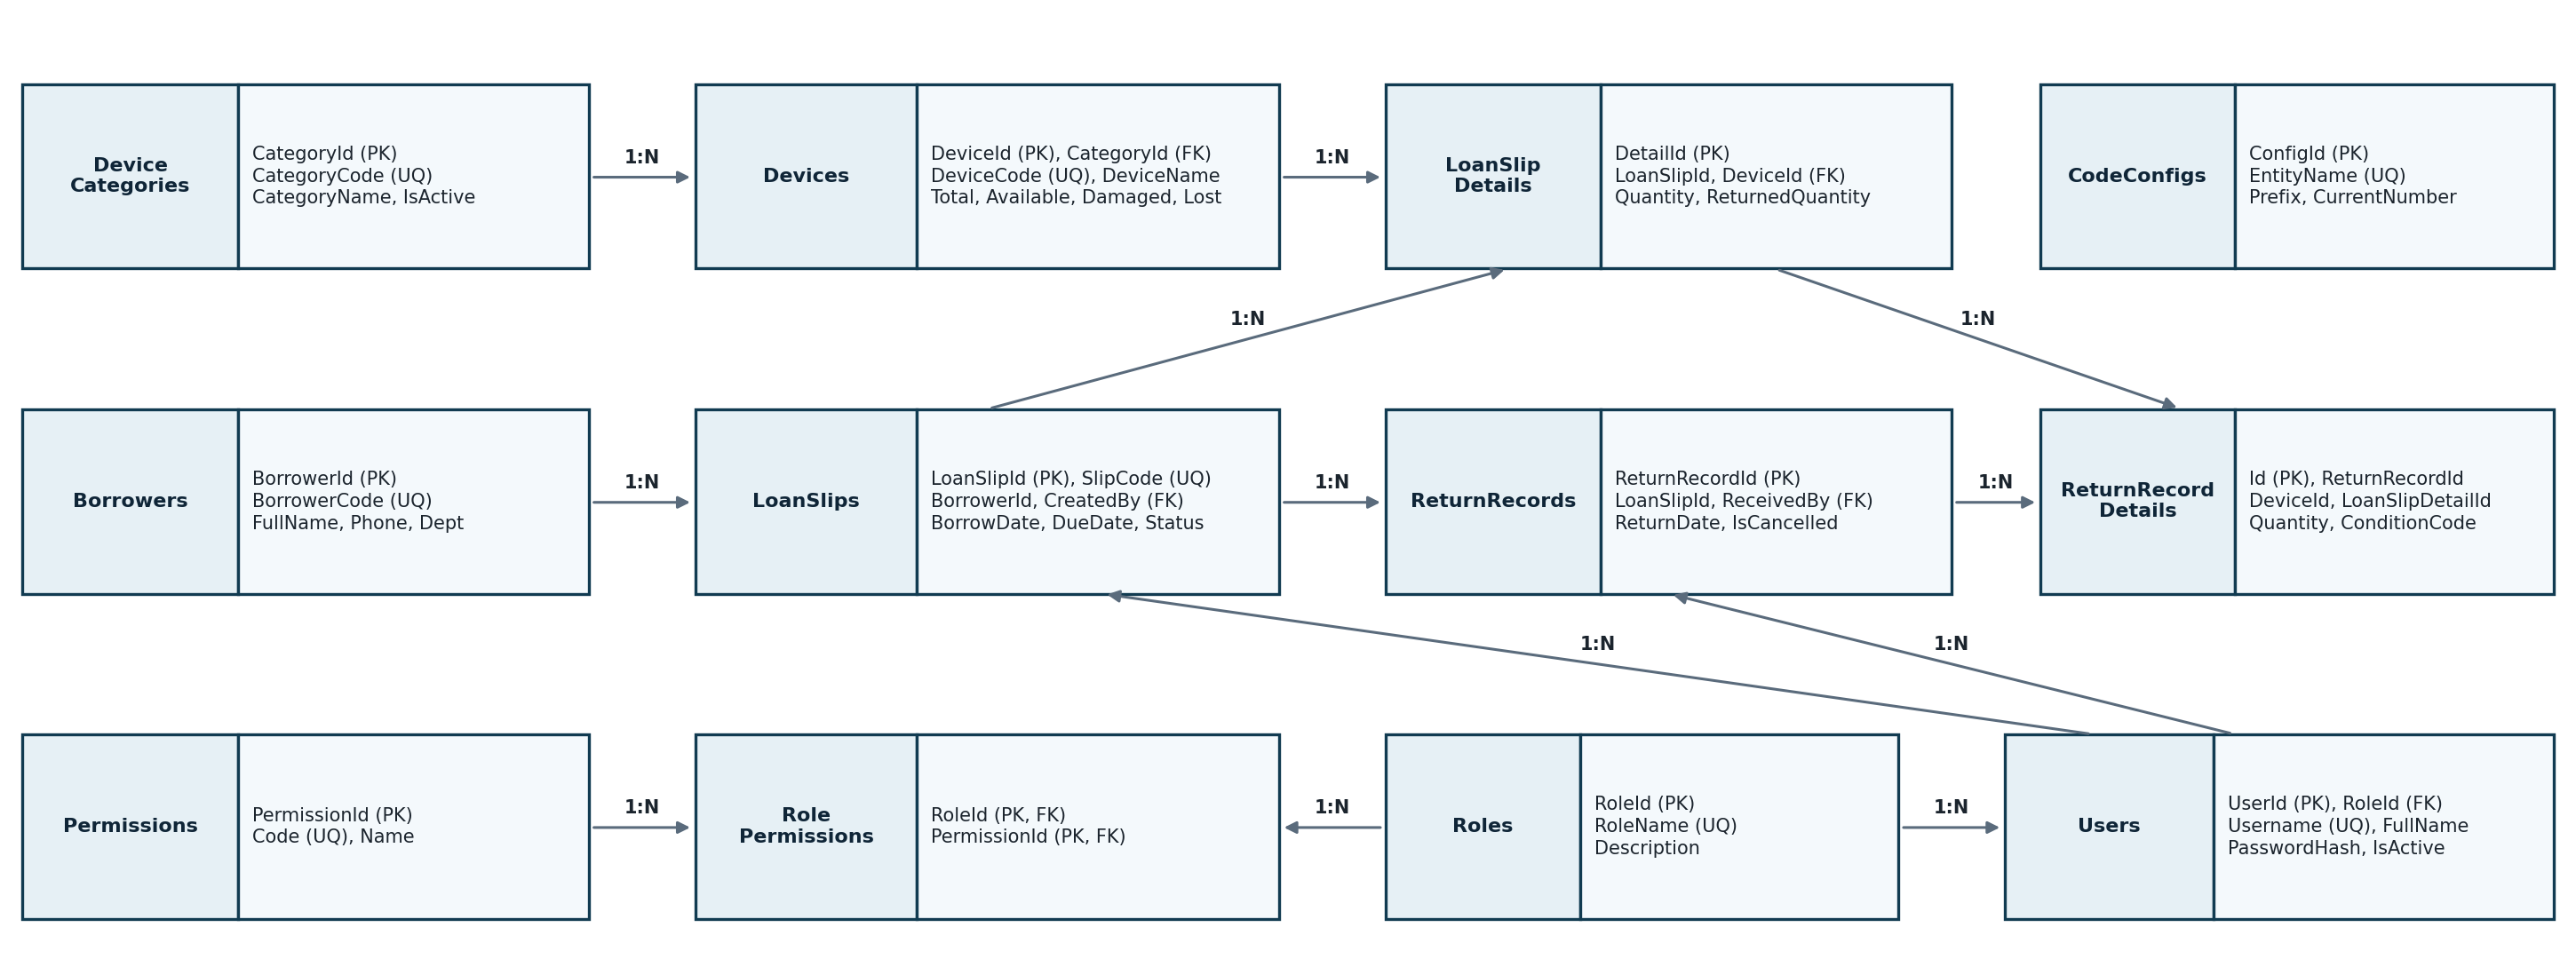
\includegraphics[width=0.8\linewidth]{images/image20.png}\caption{Sơ đồ quan hệ thực thể (ERD) hệ thống Quản lý mượn trả thiết bị}\end{figure}

\subsection{Mô tả chi tiết các bảng dữ liệu}

{\small\setlength{\tabcolsep}{3pt}\renewcommand{\arraystretch}{1.25}
\begin{longtable}{|>{\raggedright\arraybackslash}p{0.114\linewidth}|>{\raggedright\arraybackslash}p{0.133\linewidth}|>{\raggedright\arraybackslash}p{0.361\linewidth}|>{\raggedright\arraybackslash}p{0.361\linewidth}|}
\caption{Tóm tắt 12 bảng dữ liệu chính}\\
\hline
\rowcolor{gray!25}\textbf{\textbf{Bảng}} & \textbf{\textbf{Khóa chính}} & \textbf{\textbf{Trường tiêu biểu}} & \textbf{\textbf{Ý nghĩa}} \\ \hline
\endfirsthead
\hline
\rowcolor{gray!25}\textbf{\textbf{Bảng}} & \textbf{\textbf{Khóa chính}} & \textbf{\textbf{Trường tiêu biểu}} & \textbf{\textbf{Ý nghĩa}} \\ \hline
\endhead
\hline\endfoot
Roles & RoleId & RoleName (UQ), Description & Lưu danh sách vai trò/nhóm quyền trong hệ thống. \\ \hline
Permissions & PermissionId & Code (UQ), Name & Danh mục 17 mã quyền chức năng chuẩn của phần mềm. \\ \hline
RolePermissions & (RoleId, PermissionId) & RoleId (FK), PermissionId (FK) & Bảng trung gian ánh xạ quan hệ nhiều–nhiều giữa vai trò và quyền. \\ \hline
Users & UserId & Username (UQ), PasswordHash, FullName, RoleId (FK), IsActive & Lưu tài khoản nhân viên kho và người quản lý; mật khẩu băm PBKDF2. \\ \hline
DeviceCategories & CategoryId & CategoryCode (UQ), CategoryName, Description, IsActive & Danh mục phân loại trang thiết bị (Laptop, Máy chiếu, Âm thanh...). \\ \hline
Devices & DeviceId & DeviceCode (UQ), DeviceName, CategoryId (FK), TotalQuantity, AvailableQuantity, DamagedQuantity, LostQuantity & Quản lý thiết bị và cân bằng 4 nhóm số lượng tồn kho. \\ \hline
Borrowers & BorrowerId & BorrowerCode (UQ), FullName, Phone, Email, Department, Address, IsActive & Hồ sơ thông tin liên hệ và đơn vị công tác của người mượn. \\ \hline
LoanSlips & LoanSlipId & SlipCode (UQ), BorrowerId (FK), CreatedBy (FK), BorrowDate, DueDate, Status & Đầu phiếu mượn thiết bị (Status: 0 = còn nợ, 1 = đã trả đủ). \\ \hline
LoanSlipDetails & DetailId & LoanSlipId (FK), DeviceId (FK), Quantity, ReturnedQuantity & Chi tiết từng thiết bị và tiến độ số lượng đã trả trong phiếu mượn. \\ \hline
ReturnRecords & ReturnRecordId & RecordCode (UQ), LoanSlipId (FK), ReturnDate, ReceivedBy (FK), GiverName, IsCancelled, CancelledBy, CancelReason & Đầu biên bản trả/bàn giao thiết bị và thông tin truy vết hủy biên bản. \\ \hline
ReturnRecordDetails & Id & ReturnRecordId (FK), DeviceId (FK), LoanSlipDetailId (FK), Quantity, ConditionCode, Condition & Chi tiết số lượng và tình trạng thiết bị trong từng lần trả (0..3). \\ \hline
CodeConfigs & ConfigId & EntityName (UQ), Prefix, UseDate, NumberLength, CurrentNumber, ResetDaily, LastResetDate & Quy tắc và bộ đếm sinh mã tự động cho từng đối tượng. \\ \hline
\end{longtable}
}

Hệ thống thiết lập các ràng buộc toàn vẹn chặt chẽ trong \code{03\_\allowbreak{}Constraints.\allowbreak{}sql}: ràng buộc \code{CK\_\allowbreak{}Devices\_\allowbreak{}Inventory} bảo đảm \code{Available\allowbreak{}Quantity \textgreater{}= 0}, \code{Damaged\allowbreak{}Quantity \textgreater{}= 0}, \code{Lost\allowbreak{}Quantity \textgreater{}= 0} và \code{Available\allowbreak{}Quantity + Damaged\allowbreak{}Quantity + Lost\allowbreak{}Quantity \textless{}= Total\allowbreak{}Quantity}; ràng buộc \code{CK\_\allowbreak{}Loan\allowbreak{}Slip\allowbreak{}Details\_\allowbreak{}Returned} kiểm soát \code{0 \textless{}= Returned\allowbreak{}Quantity \textless{}= Quantity}; ràng buộc \code{CK\_\allowbreak{}Loan\allowbreak{}Slips\_\allowbreak{}Dates} kiểm tra \code{Due\allowbreak{}Date \textgreater{}= Borrow\allowbreak{}Date}; ràng buộc \code{CK\_\allowbreak{}RRD\_\allowbreak{}Condition\allowbreak{}Code} giới hạn mã tình trạng trong tập \code{(0, 1, 2, 3)}; và ràng buộc \code{CK\_\allowbreak{}Code\allowbreak{}Configs\_\allowbreak{}Rules} bắt buộc \code{Reset\allowbreak{}Daily = 0 OR Use\allowbreak{}Date = 1} để ngăn việc đặt lại bộ đếm mỗi ngày khi mã không đính kèm ngày tháng. Bên cạnh đó, chỉ mục duy nhất \code{UQ\_\allowbreak{}Loan\allowbreak{}Slip\allowbreak{}Details\_\allowbreak{}Slip\_\allowbreak{}Device} ngăn một thiết bị xuất hiện lặp lại trên hai dòng của cùng một phiếu mượn, và 14 chỉ mục non-clustered trong \code{04\_\allowbreak{}Indexes.\allowbreak{}sql} giúp tối ưu tốc độ tìm kiếm, lọc và nối bảng.


\subsection{View, Stored procedure và transaction}

{\small\setlength{\tabcolsep}{3pt}\renewcommand{\arraystretch}{1.25}
\begin{longtable}{|>{\raggedright\arraybackslash}p{0.233\linewidth}|>{\raggedright\arraybackslash}p{0.155\linewidth}|>{\raggedright\arraybackslash}p{0.582\linewidth}|}
\caption{Các View và Stored Procedure trong cơ sở dữ liệu}\\
\hline
\rowcolor{gray!25}\textbf{\textbf{Đối tượng SQL}} & \textbf{\textbf{Loại}} & \textbf{\textbf{Mục đích và cơ chế xử lý}} \\ \hline
\endfirsthead
\hline
\rowcolor{gray!25}\textbf{\textbf{Đối tượng SQL}} & \textbf{\textbf{Loại}} & \textbf{\textbf{Mục đích và cơ chế xử lý}} \\ \hline
\endhead
\hline\endfoot
vw\_LoanSlipSummary & View & Tổng hợp đầu phiếu mượn, thông tin người mượn, người lập, tổng số lượng mượn (TotalQty), đã trả (ReturnedQty), còn lại (RemainingQty), số ngày trễ (DaysOverdue) và tự động suy diễn trạng thái hiển thị DisplayStatus (0: Đang mượn, 1: Trả một phần, 2: Đã trả, 3: Quá hạn). \\ \hline
sp\_GetNextCode & Stored Procedure & Sinh mã tự động theo bảng CodeConfigs. Sử dụng gợi ý khóa dòng WITH (UPDLOCK, HOLDLOCK) trong transaction để nhiều người dùng thao tác cùng lúc không bao giờ sinh trùng mã; hỗ trợ chế độ @Peek = 1 để xem trước mã mà không tăng bộ đếm. \\ \hline
sp\_GetOverdueSlips & Stored Procedure & Truy vấn danh sách phiếu quá hạn thực tế theo ngày (@AsOfDate), hỗ trợ lọc từ khóa (@Keyword) và số ngày quá hạn tối thiểu (@MinDaysOverdue), đồng thời dùng CROSS APPLY + STRING\_AGG để nối danh sách tên thiết bị và số lượng chưa trả. \\ \hline
sp\_RecalculateInventory & Stored Procedure & Đồng bộ lại trạng thái phiếu mượn (LoanSlips.Status) và tính lại tồn kho khả dụng chuẩn xác theo công thức Available = Total - (Đang mượn) - Damaged - Lost; dùng sau khi nạp dữ liệu mẫu hoặc khi cần đối soát dữ liệu. \\ \hline
\end{longtable}
}

\section{Kiến trúc và luồng xử lý}

Ứng dụng được tổ chức thành 2 project trong cùng một solution: \code{Quan\allowbreak{}Ly\allowbreak{}Muon\allowbreak{}Tra.\allowbreak{}UI} (thư viện control và chủ đề giao diện) và \code{Quan\allowbreak{}Ly\allowbreak{}Muon\allowbreak{}Tra.\allowbreak{}App} (chứa các phân lớp \code{Forms}/\code{Pages}, \code{Services}, \code{Data}, \code{Models}, \code{Security}). Hình 3.2 minh họa kiến trúc MVP và mối liên hệ giữa các thành phần và Hình 3.3 thể hiện luồng xử lý nghiệp vụ mượn – trả thiết bị khép kín.


\begin{figure}[H]\centering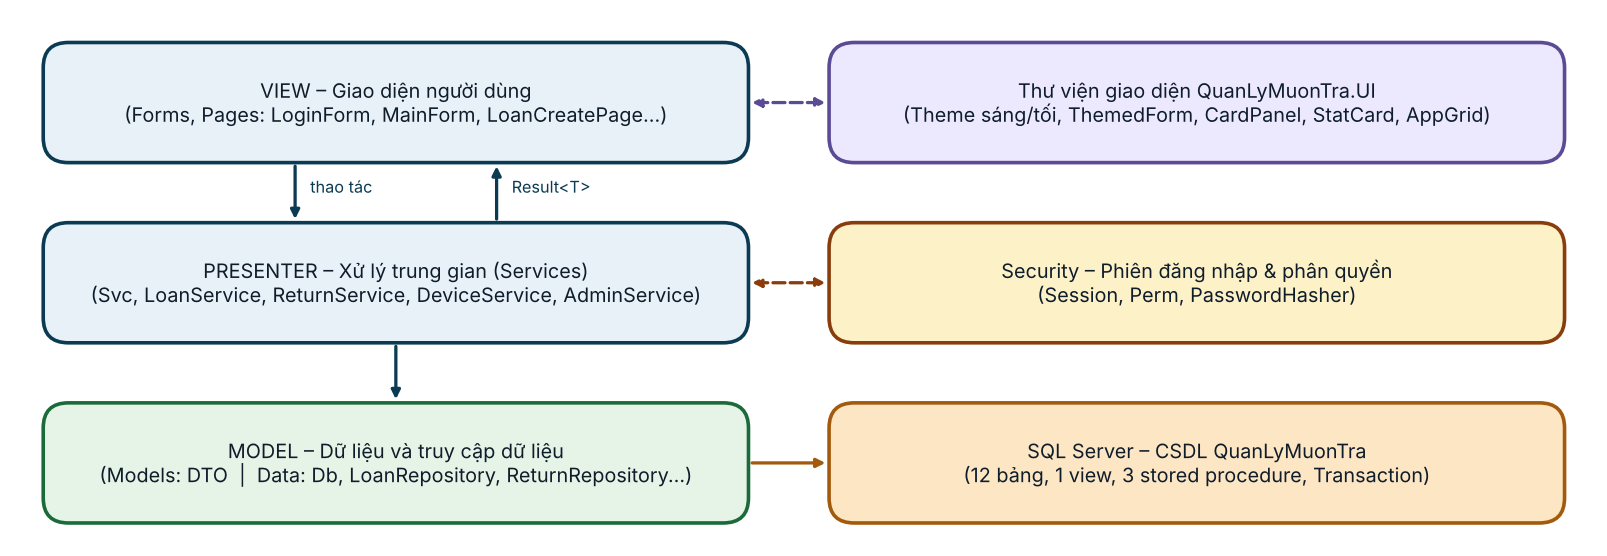
\includegraphics[width=0.8\linewidth]{images/image21.png}\caption{Mô hình kiến trúc MVP (Model – View – Presenter), SQL Server và thư viện UI}\end{figure}

\begin{figure}[H]\centering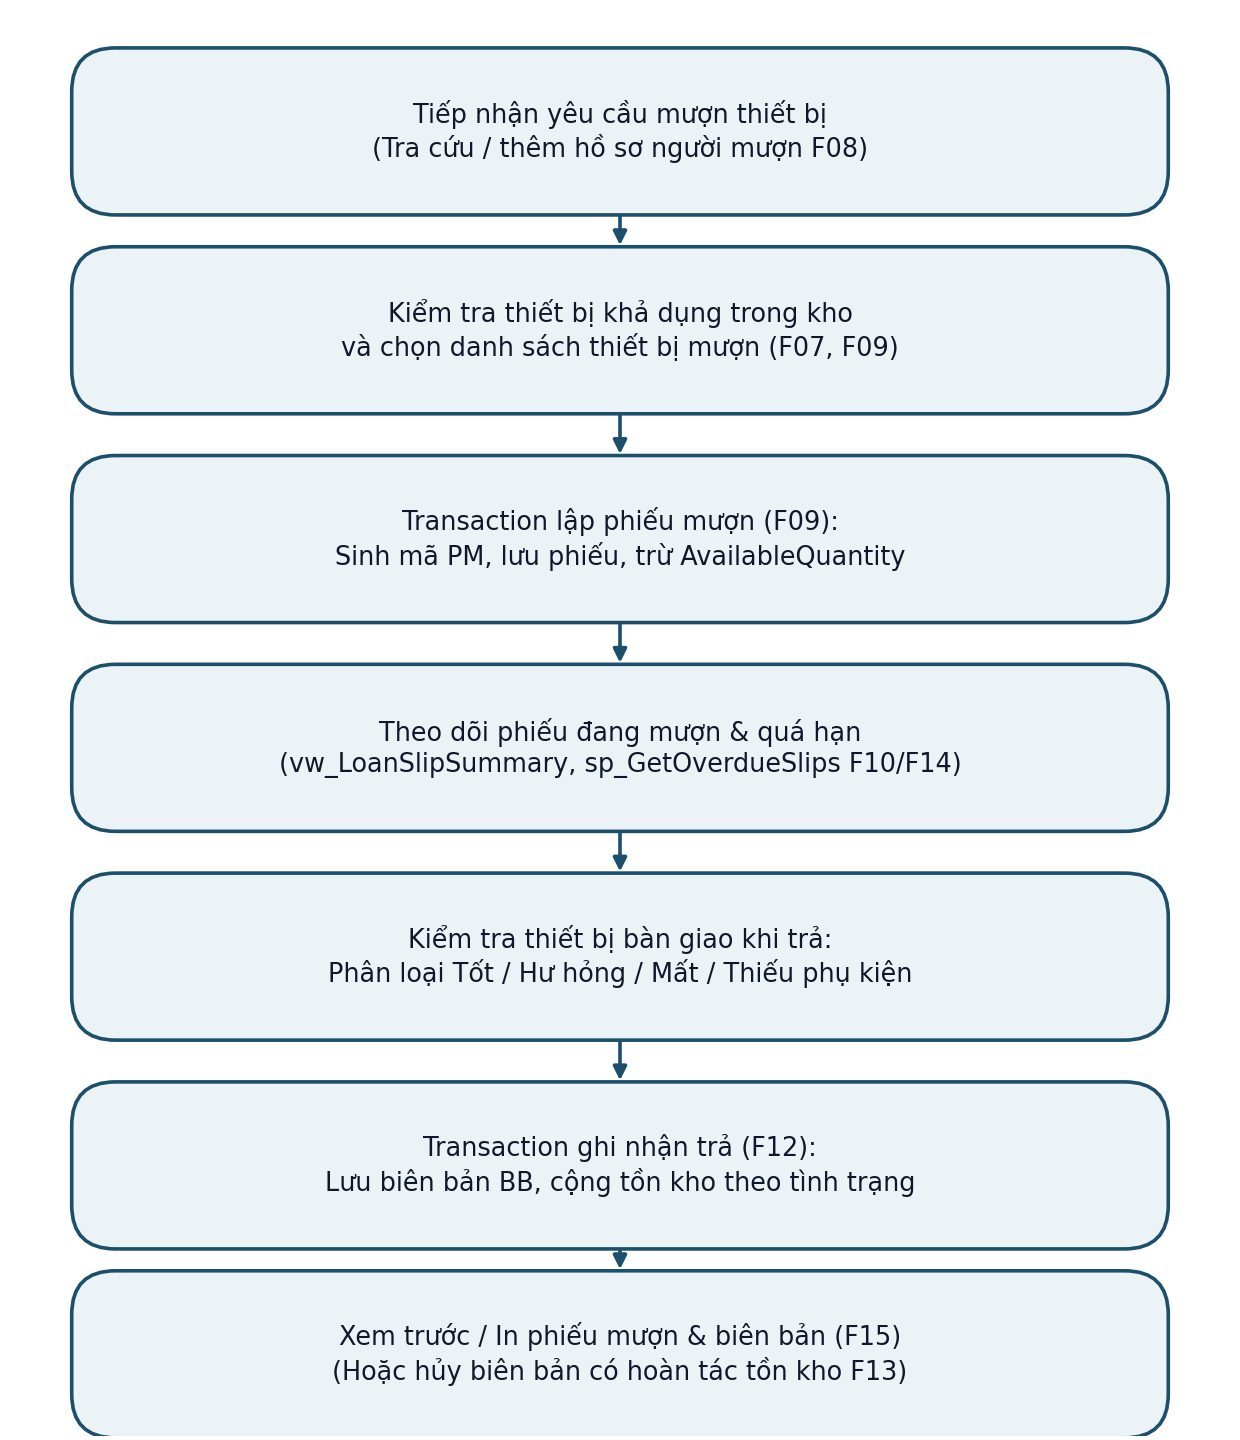
\includegraphics[width=0.8\linewidth]{images/image22.png}\caption{Quy trình nghiệp vụ từ lập phiếu mượn đến ghi nhận trả và in biên bản}\end{figure}

\section{Quy tắc nghiệp vụ và kiểm soát tồn kho}

Khác với bài toán bán hàng thông thường, bài toán quản lý mượn trả thiết bị đòi hỏi bảo toàn tổng số lượng tài sản đầu tư trong suốt vòng đời cho mượn, trả lại, hư hỏng, sửa chữa hoặc thất lạc. Các công thức bất biến được duy trì xuyên suốt giữa tầng C\# (\code{Loan\allowbreak{}Repository.\allowbreak{}cs}, \code{Return\allowbreak{}Repository.\allowbreak{}cs}) và tầng SQL Server (\code{03\_\allowbreak{}Constraints.\allowbreak{}sql}, \code{05\_\allowbreak{}Stored\allowbreak{}Procedures.\allowbreak{}sql}):


\begin{Verbatim}
ĐangMượn (OnLoanQuantity) = Σ (Quantity - ReturnedQuantity) trên LoanSlipDetails
TổngSốLượng (TotalQuantity) = AvailableQuantity + OnLoanQuantity + DamagedQuantity + LostQuantity
CònPhảiTrả (RemainingQty) = TotalQty - ReturnedQty (trên từng dòng và toàn phiếu)
SốNgàyQuáHạn (DaysOverdue) = max(0, (HômNay - DueDate).Days) khi RemainingQty > 0 và DueDate < HômNay
\end{Verbatim}

Khi ghi nhận trả thiết bị tại \code{Return\allowbreak{}Repository.\allowbreak{}Create}, phương thức phân loại \code{Bucket(condition\allowbreak{}Code, qty)} quy đổi số lượng trả vào 3 rổ tồn kho \code{(Good, Damaged, Lost)} theo đúng mã tình trạng: nếu trả ở tình trạng \textbf{Tốt (\code{0})}, số lượng được cộng trả lại vào \code{Available\allowbreak{}Quantity} để sẵn sàng cho lượt mượn tiếp theo; nếu trả ở tình trạng \textbf{Hư hỏng (\code{1})} hoặc \textbf{Thiếu phụ kiện (\code{3})}, số lượng được cộng vào \code{Damaged\allowbreak{}Quantity} (chờ sửa chữa/bổ sung phụ kiện qua \code{Recover\allowbreak{}Damaged}); nếu trả ở tình trạng \textbf{Mất (\code{2})}, số lượng được cộng vào \code{Lost\allowbreak{}Quantity}. Trạng thái hiển thị \code{Display\allowbreak{}Status} của phiếu mượn không lưu cứng mà được tính động trên \code{vw\_\allowbreak{}Loan\allowbreak{}Slip\allowbreak{}Summary}: ưu tiên kiểm tra nếu \code{Remaining\allowbreak{}Qty = 0} là \code{Đã trả (2)}, ngược lại nếu \code{Due\allowbreak{}Date \textless{} Hôm\allowbreak{}Nay} là \code{Quá hạn (3)}, nếu \code{Returned\allowbreak{}Qty \textgreater{} 0} là \code{Trả một phần (1)}, và mặc định là \code{Đang mượn (0)}.


{\small\setlength{\tabcolsep}{3pt}\renewcommand{\arraystretch}{1.25}
\begin{longtable}{|>{\raggedright\arraybackslash}p{0.485\linewidth}|>{\raggedright\arraybackslash}p{0.485\linewidth}|}
\caption{Các tình huống kiểm soát nghiệp vụ}\\
\hline
\rowcolor{gray!25}\textbf{\textbf{Tình huống nghiệp vụ}} & \textbf{\textbf{Cơ chế kiểm soát và kết quả kỳ vọng}} \\ \hline
\endfirsthead
\hline
\rowcolor{gray!25}\textbf{\textbf{Tình huống nghiệp vụ}} & \textbf{\textbf{Cơ chế kiểm soát và kết quả kỳ vọng}} \\ \hline
\endhead
\hline\endfoot
Hai nhân viên cùng mượn một thiết bị sắp hết tồn & Câu lệnh UPDATE Devices ... WHERE AvailableQuantity \textgreater{}= @qty chỉ khớp cho giao dịch đến trước; giao dịch đến sau nhận rows = 0, ném BusinessException và rollback toàn bộ phiếu. \\ \hline
Chọn trùng một thiết bị nhiều lần trên cùng phiếu mượn & Giao diện cộng dồn số lượng trong giỏ; lớp Data (thuộc Model) dùng GroupBy(i =\textgreater{} i.DeviceId).OrderBy(g =\textgreater{} g.Key) gộp thành 1 dòng duy nhất và khóa theo thứ tự ID cố định để tránh Deadlock. \\ \hline
Trả vượt quá số lượng còn phải trả của dòng phiếu & ReturnRepository khóa phiếu bằng WITH (UPDLOCK, HOLDLOCK), đối chiếu tổng số lượng trả với (Quantity - ReturnedQuantity); nếu vượt sẽ từ chối và rollback. \\ \hline
Trả thiết bị hư hỏng hoặc thiếu phụ kiện nhưng bỏ trống ghi chú & ReturnService.Validate bắt buộc nhập ConditionNote chi tiết khi Condition là Damaged hoặc MissingAccessory; từ chối lưu nếu để trống. \\ \hline
Hủy biên bản trả sau khi thiết bị vừa trả đã được cho mượn lại & ReturnRepository.Cancel kiểm tra AvailableQuantity \textgreater{}= @good AND DamagedQuantity \textgreater{}= @damaged AND LostQuantity \textgreater{}= @lost; nếu tồn kho hiện tại không đủ để trừ hoàn tác thì từ chối hủy. \\ \hline
Bật đặt lại bộ đếm mã hằng ngày nhưng không chèn ngày vào mã & AdminService.SaveCodeConfig và CK\_CodeConfigs\_Rules chặn cấu hình (ResetDaily = 1 khi UseDate = 0) nhằm ngăn sinh trùng mã vào ngày hôm sau. \\ \hline
\end{longtable}
}

\section{Ma trận phân quyền người dùng}

Trong kịch bản khởi tạo \code{06\_\allowbreak{}Seed\allowbreak{}Data.\allowbreak{}sql}, hệ thống định nghĩa sẵn 17 mã quyền chức năng và 2 vai trò mẫu: \textbf{Người quản lý} (được gán toàn bộ 17 quyền) và \textbf{Nhân viên kho} (được gán 10 quyền phục vụ công việc vận hành kho hằng ngày). Người quản lý có thể thay đổi tập quyền này bất kỳ lúc nào trên màn hình F05.


{\small\setlength{\tabcolsep}{3pt}\renewcommand{\arraystretch}{1.25}
\begin{longtable}{|>{\raggedright\arraybackslash}p{0.240\linewidth}|>{\raggedright\arraybackslash}p{0.472\linewidth}|>{\raggedright\arraybackslash}p{0.129\linewidth}|>{\raggedright\arraybackslash}p{0.129\linewidth}|}
\caption{Ma trận phân quyền mặc định theo hai vai trò}\\
\hline
\rowcolor{gray!25}\textbf{\textbf{Mã quyền (Permission Code)}} & \textbf{\textbf{Tên quyền chức năng}} & \textbf{\textbf{Nhân viên kho}} & \textbf{\textbf{Người quản lý}} \\ \hline
\endfirsthead
\hline
\rowcolor{gray!25}\textbf{\textbf{Mã quyền (Permission Code)}} & \textbf{\textbf{Tên quyền chức năng}} & \textbf{\textbf{Nhân viên kho}} & \textbf{\textbf{Người quản lý}} \\ \hline
\endhead
\hline\endfoot
DASHBOARD\_VIEW & Xem màn hình Tổng quan (Dashboard F02) & Có & Có \\ \hline
CATEGORY\_VIEW & Xem danh mục loại thiết bị (F06) & Có & Có \\ \hline
CATEGORY\_MANAGE & Thêm, sửa, xóa loại thiết bị (F06) & Không & Có \\ \hline
DEVICE\_MANAGE & Quản lý thiết bị và phục hồi hư hỏng (F07) & Có & Có \\ \hline
BORROWER\_MANAGE & Quản lý hồ sơ người mượn và lịch sử (F08) & Có & Có \\ \hline
LOAN\_CREATE & Lập phiếu mượn thiết bị (F09) & Có & Có \\ \hline
LOAN\_VIEW & Tra cứu và xem chi tiết phiếu mượn (F10, F11) & Có & Có \\ \hline
RETURN\_CREATE & Ghi nhận trả thiết bị (F12) & Có & Có \\ \hline
RECORD\_VIEW & Tra cứu và xem chi tiết biên bản trả (F13) & Có & Có \\ \hline
RECORD\_CANCEL & Hủy biên bản trả / bàn giao (F13) & Không & Có \\ \hline
OVERDUE\_VIEW & Xem danh sách phiếu quá hạn (F14) & Có & Có \\ \hline
REPORT\_PRINT & Xem trước và in phiếu mượn, biên bản trả (F15) & Có & Có \\ \hline
REPORT\_VIEW & Xem số liệu báo cáo tổng hợp mượn trả \& tồn kho (F15) & Không & Có \\ \hline
STATS\_VIEW & Xem thống kê thiết bị được mượn nhiều (F18) & Không & Có \\ \hline
USER\_MANAGE & Quản lý tài khoản, khóa/mở khóa, đặt lại mật khẩu (F04) & Không & Có \\ \hline
ROLE\_MANAGE & Quản lý nhóm quyền và gán quyền chức năng (F05) & Không & Có \\ \hline
CODE\_CONFIG & Cấu hình quy tắc sinh mã tự động (F16) & Không & Có \\ \hline
\end{longtable}
}

\chapter{TRIỂN KHAI VÀ KẾT QUẢ}

\section{Môi trường phát triển}

{\small\setlength{\tabcolsep}{3pt}\renewcommand{\arraystretch}{1.25}
\begin{longtable}{|>{\raggedright\arraybackslash}p{0.277\linewidth}|>{\raggedright\arraybackslash}p{0.693\linewidth}|}
\caption{Công nghệ và môi trường triển khai}\\
\hline
\rowcolor{gray!25}\textbf{\textbf{Thành phần}} & \textbf{\textbf{Công nghệ hoặc yêu cầu}} \\ \hline
\endfirsthead
\hline
\rowcolor{gray!25}\textbf{\textbf{Thành phần}} & \textbf{\textbf{Công nghệ hoặc yêu cầu}} \\ \hline
\endhead
\hline\endfoot
Hệ điều hành & Windows 10 / Windows 11 (64-bit) \\ \hline
Ngôn ngữ \& Nền tảng & C\# trên .NET 10 (target framework: net10.0-windows) \\ \hline
Công cụ phát triển (IDE) & Visual Studio 2022 / 2026 có workload .NET desktop development \\ \hline
Giao diện Desktop (UI) & Windows Forms + Thư viện tự xây dựng QuanLyMuonTra.UI (GDI+, Segoe MDL2 Assets) \\ \hline
Hệ quản trị CSDL & Microsoft SQL Server 2017 trở lên (Express / Developer / LocalDB) \\ \hline
Truy cập dữ liệu (Model/Data) & Dapper 2.x kết hợp Microsoft.Data.SqlClient 6.x (ADO.NET) \\ \hline
Bảo mật mật khẩu & PBKDF2-SHA256 (100.000 vòng lặp, Salt 16 byte, Key 32 byte) \\ \hline
In ấn biểu mẫu & System.Drawing.Printing (PrintDocument \& PrintPreviewDialog) \\ \hline
Quản lý cấu hình & Tệp văn bản connection.txt đặt cạnh tệp thực thi (.exe) \\ \hline
\end{longtable}
}

\section{Cấu trúc Project}

\subsection{Sơ đồ tổng quan cấu trúc thư mục}

\begin{Verbatim}
QuanLyMuonTra.slnx
|-- QuanLyMuonTra.UI/        (Thư viện control & chủ đề Sáng/Tối)
|   |-- Theme.cs, ThemedBase.cs, Surfaces.cs
|   `-- Inputs.cs, Widgets.cs, Gfx.cs
|-- QuanLyMuonTra.App/       (Ứng dụng chính Windows Forms)
|   |-- Forms/               (LoginForm, MainForm, PrintHelper & 10 Dialog)
|   |-- Pages/               (14 UserControl chức năng F02, F04–F16, F18)
|   |-- Services/            (Presenter: nghiệp vụ & kiểm tra quyền)
|   |-- Data/                (Model: truy vấn SQL Server với Dapper)
|   |-- Models/              (DTO và các lớp bộ lọc truy vấn)
|   |-- Security/            (Session.cs, Perm.cs, PasswordHasher.cs)
|   |-- NavCatalog.cs, Program.cs, connection.txt
|-- Database/                (01_CreateDatabase.sql -> 07_TestData.sql)
`-- docs/                    (TEST_CASES.md, BAO_CAO_NHOM_TEMPLATE.md...)
\end{Verbatim}

\subsection{Vai trò của các thành phần}

\code{Program.\allowbreak{}cs} khởi tạo cấu hình ứng dụng và chạy vòng lặp xác thực: mở \code{Login\allowbreak{}Form} để đăng nhập, nếu thành công thì khởi chạy \code{Main\allowbreak{}Form}; nếu người dùng nhấn \code{Đăng xuất} (\code{main.\allowbreak{}Logged\allowbreak{}Out == true}), chương trình xóa phiên \code{Session.\allowbreak{}End()} và quay lại \code{Login\allowbreak{}Form} mà không cần tắt ứng dụng. Các lớp trong \code{Pages/\allowbreak{}} đảm nhiệm từng màn hình nghiệp vụ lớn được nhúng vào \code{Main\allowbreak{}Form}, trong khi các hộp thoại trong \code{Forms/\allowbreak{}} (\code{Device\allowbreak{}Edit\allowbreak{}Dialog}, \code{Borrower\allowbreak{}Edit\allowbreak{}Dialog}, \code{Loan\allowbreak{}Slip\allowbreak{}Detail\allowbreak{}Dialog}, \code{Return\allowbreak{}Create\allowbreak{}Dialog}...) xử lý tác vụ nhập liệu hoặc xem chi tiết chuyên sâu.


\section{Cấu hình và chạy chương trình}

Bước 1: Cài đặt .NET 10 SDK, Visual Studio (có workload .NET desktop development) và Microsoft SQL Server (2017 trở lên). Bước 2: Mở SQL Server Management Studio (SSMS), kết nối tới SQL Server và chạy lần lượt các tập lệnh trong thư mục \code{Database/\allowbreak{}} theo đúng thứ tự từ \code{01\_\allowbreak{}Create\allowbreak{}Database.\allowbreak{}sql} đến \code{06\_\allowbreak{}Seed\allowbreak{}Data.\allowbreak{}sql} (và \code{07\_\allowbreak{}Test\allowbreak{}Data.\allowbreak{}sql} nếu muốn nạp 5 phiếu mượn và 3 biên bản kiểm thử). Bước 3: Mở tệp \code{Quan\allowbreak{}Ly\allowbreak{}Muon\allowbreak{}Tra.\allowbreak{}App/\allowbreak{}connection.\allowbreak{}txt} và cập nhật chuỗi kết nối phù hợp với máy tính triển khai:


\begin{Verbatim}
Server=.\SQLEXPRESS;Database=QuanLyMuonTra;Trusted_Connection=True;TrustServerCertificate=True;
\end{Verbatim}

Bước 4: Mở solution \code{Quan\allowbreak{}Ly\allowbreak{}Muon\allowbreak{}Tra.\allowbreak{}slnx} bằng Visual Studio hoặc sử dụng dòng lệnh .NET CLI để khôi phục gói NuGet, biên dịch và chạy ứng dụng:


\begin{Verbatim}
dotnet restore .\QuanLyMuonTra.slnx
dotnet build .\QuanLyMuonTra.slnx
dotnet run --project .\QuanLyMuonTra.App\QuanLyMuonTra.App.csproj
\end{Verbatim}

Bước 5: Đăng nhập thử nghiệm bằng hai tài khoản mẫu được tạo sẵn trong \code{06\_\allowbreak{}Seed\allowbreak{}Data.\allowbreak{}sql}: tài khoản Người quản lý (\code{admin} / \code{Admin@123}) hoặc tài khoản Nhân viên kho (\code{kho01} / \code{Kho@123}).


\section{Chi tiết các chức năng quan trọng}

\subsection{Kiểm soát truy cập, băm mật khẩu và phân quyền động}

Quá trình xác thực tại \code{User\allowbreak{}Repository.\allowbreak{}Authenticate} truy vấn thông tin người dùng theo \code{Username}, kiểm tra mật khẩu thông qua \code{Password\allowbreak{}Hasher.\allowbreak{}Verify} (PBKDF2-SHA256 100.000 vòng lặp) và kiểm tra trạng thái \code{Is\allowbreak{}Active}. Nếu hợp lệ, danh sách mã quyền của vai trò tương ứng được nạp vào \code{Session}. Mọi phương thức ở Presenter (\code{Services}) đều đi qua hàm bọc \code{Svc.\allowbreak{}Run(permissions, work)}: nếu người dùng chưa đăng nhập hoặc không sở hữu ít nhất một quyền trong mảng yêu cầu, hàm lập tức trả về \code{Result.\allowbreak{}Fail("Bạn không có quyền thực hiện chức năng này.\allowbreak{}")} trước khi chạm tới cơ sở dữ liệu.


\hinhanh{hinh4_01_login}{Giao diện đăng nhập và thông báo kiểm tra tài khoản/mật khẩu}{Nội dung cần chụp: Màn hình đăng nhập (LoginForm) khi nhập tài khoản admin/kho01 hoặc khi thông báo lỗi sai mật khẩu / tài khoản bị khóa\\[2pt] (Thành phần mã nguồn: QuanLyMuonTra.App/Forms/LoginForm.cs)}

\subsection{Lập phiếu mượn nhiều thiết bị và trừ tồn kho có điều kiện}

Tại \code{Loan\allowbreak{}Create\allowbreak{}Page}, nhân viên có thể tìm kiếm nhanh các thiết bị còn tồn kho, chọn số lượng và thêm nhiều thiết bị vào giỏ mượn. Khi lưu phiếu, \code{Loan\allowbreak{}Service.\allowbreak{}Validate} kiểm tra người mượn hợp lệ, ngày mượn không ở tương lai (\code{Borrow\allowbreak{}Date \textless{}= Today}), hạn trả không trước ngày mượn (\code{Due\allowbreak{}Date \textgreater{}= Borrow\allowbreak{}Date}) và số lượng mỗi dòng lớn hơn 0. Tiếp đó, \code{Loan\allowbreak{}Repository.\allowbreak{}Create} mở transaction qua \code{Db.\allowbreak{}In\allowbreak{}Transaction}, sinh mã phiếu mới bằng \code{Code\allowbreak{}Repository.\allowbreak{}Next}, tạo bản ghi \code{Loan\allowbreak{}Slips} và duyệt qua từng thiết bị theo thứ tự \code{Device\allowbreak{}Id} tăng dần. Câu lệnh \code{UPDATE Devices SET Available\allowbreak{}Quantity = Available\allowbreak{}Quantity -\allowbreak{} @qty WHERE Device\allowbreak{}Id = @device\allowbreak{}Id AND Is\allowbreak{}Active = 1 AND Available\allowbreak{}Quantity \textgreater{}= @qty} bảo đảm việc kiểm tra và trừ tồn diễn ra nguyên tử (atomic); nếu \code{rows == 0}, toàn bộ giao dịch lập tức rollback.


\hinhanh{hinh4_02_lapphieu}{Giao diện lập phiếu mượn nhiều thiết bị và giỏ thiết bị (F09)}{Nội dung cần chụp: Màn hình Lập phiếu mượn (LoanCreatePage) với danh sách thiết bị khả dụng bên trái và giỏ thiết bị chọn mượn bên phải\\[2pt] (Thành phần mã nguồn: QuanLyMuonTra.App/Pages/LoanCreatePage.cs)}

\subsection{Ghi nhận trả theo tình trạng và hoàn tác khi hủy biên bản}

Nghiệp vụ trả thiết bị (\code{Return\allowbreak{}Create\allowbreak{}Dialog} và \code{Return\allowbreak{}Repository.\allowbreak{}Create}) cho phép người mượn trả từng phần hoặc trả toàn bộ thiết bị trên phiếu, đồng thời cho phép tách một thiết bị thành các dòng trạng thái khác nhau (Tốt, Hư hỏng, Mất, Thiếu phụ kiện). Trong transaction, hệ thống khóa dòng \code{Loan\allowbreak{}Slips} và \code{Loan\allowbreak{}Slip\allowbreak{}Details} bằng \code{WITH (UPDLOCK, HOLDLOCK)}, kiểm tra tổng số lượng trả của từng mục không vượt số lượng còn nợ (\code{Quantity -\allowbreak{} Returned\allowbreak{}Quantity}), tạo biên bản \code{Return\allowbreak{}Records} + \code{Return\allowbreak{}Record\allowbreak{}Details}, tăng \code{Returned\allowbreak{}Quantity} và phân bổ số lượng vào đúng cột \code{Available\allowbreak{}Quantity}, \code{Damaged\allowbreak{}Quantity} hoặc \code{Lost\allowbreak{}Quantity}. Cuối cùng, câu lệnh \code{Recompute\allowbreak{}Status\allowbreak{}Sql} tự động chuyển \code{Loan\allowbreak{}Slips.\allowbreak{}Status = 1} nếu toàn bộ các dòng trong phiếu đã được trả đủ. Khi cần hủy một biên bản lập nhầm (\code{Return\allowbreak{}Repository.\allowbreak{}Cancel}), hệ thống kiểm tra tồn kho hiện tại có đủ để trừ ngược hay không trước khi hoàn tác và đánh dấu \code{Is\allowbreak{}Cancelled = 1}.


\hinhanh{hinh4_03_ghinhantra}{Hộp thoại ghi nhận trả thiết bị theo tình trạng (F12)}{Nội dung cần chụp: Hộp thoại Ghi nhận trả (ReturnCreateDialog) hiển thị số lượng còn phải trả, cột chọn Tình trạng (Tốt/Hư hỏng/Mất/Thiếu phụ kiện) và ghi chú\\[2pt] (Thành phần mã nguồn: QuanLyMuonTra.App/Forms/ReturnCreateDialog.cs)}

\hinhanh{hinh4_04_inpreview}{Cửa sổ xem trước bản in phiếu mượn và biên bản bàn giao (F15)}{Nội dung cần chụp: Cửa sổ PrintPreviewDialog hiển thị mẫu in Phiếu mượn thiết bị hoặc Biên bản trả / bàn giao thiết bị kèm phần chữ ký\\[2pt] (Thành phần mã nguồn: QuanLyMuonTra.App/Forms/PrintHelper.cs)}

\subsection{Báo cáo tổng hợp, thống kê thiết bị mượn nhiều và in ấn}

Chức năng báo cáo (\code{Report\allowbreak{}Page} và \code{Admin\allowbreak{}Repository.\allowbreak{}Summary}) tổng hợp đồng thời các chỉ số giao dịch trong kỳ lọc (\code{Slip\allowbreak{}Count}, \code{Borrowed\allowbreak{}Quantity}, \code{Returned\allowbreak{}Quantity}, \code{Outstanding\allowbreak{}Quantity}, \code{Overdue\allowbreak{}Slip\allowbreak{}Count}) và các chỉ số tồn kho hiện hành (\code{Active\allowbreak{}Device\allowbreak{}Count}, \code{Available\allowbreak{}Quantity}, \code{Damaged\allowbreak{}Quantity}, \code{Lost\allowbreak{}Quantity}), kết hợp hiển thị bảng xếp hạng Top thiết bị được mượn nhiều nhất. Đối với chức năng thống kê chuyên sâu (\code{Popular\allowbreak{}Device\allowbreak{}Page} – F18), người dùng có thể tùy chỉnh khoảng ngày và giới hạn \code{Top N} (từ 1 đến 100) để phân tích nhu cầu sử dụng thiết bị thực tế.


\hinhanh{hinh4_05_baocao}{Màn hình báo cáo tổng hợp và thống kê thiết bị mượn nhiều (F15, F18)}{Nội dung cần chụp: Màn hình Báo cáo \& in ấn (ReportPage) hoặc Thiết bị mượn nhiều (PopularDevicePage) với các chỉ số tổng hợp dưới chân trang\\[2pt] (Thành phần mã nguồn: QuanLyMuonTra.App/Pages/ReportPage.cs, PopularDevicePage.cs)}

\subsection{Sinh mã tự động an toàn đồng thời và chế độ sáng/tối}

Màn hình \code{Code\allowbreak{}Config\allowbreak{}Page} (F16) quản lý bảng \code{Code\allowbreak{}Configs} và kết nối với thủ tục \code{dbo.\allowbreak{}sp\_\allowbreak{}Get\allowbreak{}Next\allowbreak{}Code}. Khi người dùng nhấn \code{Xem mã tiếp theo}, hệ thống gọi \code{Code\allowbreak{}Repository.\allowbreak{}Peek} (\code{@Peek = 1}) để hiển thị chuỗi mã dự kiến (ví dụ \code{PM-\allowbreak{}20261107-\allowbreak{}0001} hoặc \code{TB0009}) mà không làm tăng bộ đếm trong cơ sở dữ liệu. Ngoài ra, khi người dùng tự nhập tay mã thiết bị dạng \code{TB0012}, hàm \code{Code\allowbreak{}Repository.\allowbreak{}Sync\allowbreak{}Counter} tự động kéo \code{Current\allowbreak{}Number} lên theo số lớn nhất để các lần gợi ý sau không bị trùng. Về trải nghiệm thị giác, lớp \code{Theme} và \code{Theme\allowbreak{}Applier} cho phép chuyển đổi tức thời giữa giao diện Sáng (\code{\#F5F7FA} / \code{\#FFFFFF}) và giao diện Tối (\code{\#0F172A} / \code{\#1E293B}) ngay trên thanh tiêu đề.


\hinhanh{hinh4_06_cauhinhma}{Màn hình cấu hình quy tắc sinh mã tự động và xem trước mã (F16)}{Nội dung cần chụp: Màn hình Cấu hình mã tự động (CodeConfigPage) với lưới 4 đối tượng (LoanSlip, ReturnRecord, Device, Borrower) và thanh chỉnh sửa phía dưới\\[2pt] (Thành phần mã nguồn: QuanLyMuonTra.App/Pages/CodeConfigPage.cs)}

\hinhanh{hinh4_07_darkmode}{Giao diện chính khi chuyển đổi chế độ Sáng / Tối (ThemeMode)}{Nội dung cần chụp: Giao diện MainForm và nội dung trang khi kích hoạt chế độ Giao diện tối (Dark Mode)\\[2pt] (Thành phần mã nguồn: QuanLyMuonTra.UI/Theme.cs, QuanLyMuonTra.App/Forms/MainForm.cs)}

\section{Hình ảnh sản phẩm thực tế}

Các hình dưới đây là ảnh chụp màn hình thực tế khi chạy ứng dụng trên Windows, được sắp xếp theo thứ tự chức năng của hệ thống.


\hinhanh{hinh4_08_dashboard_kho}{Màn hình Tổng quan (Dashboard F02) của tài khoản Nhân viên kho}{Nội dung cần chụp: Màn hình Dashboard khi đăng nhập bằng tài khoản kho01 (chỉ hiển thị các menu được phân quyền cho nhân viên kho)\\[2pt] (Thành phần mã nguồn: QuanLyMuonTra.App/Forms/MainForm.cs, Pages/DashboardPage.cs)}

\hinhanh{hinh4_09_dashboard_admin}{Màn hình Tổng quan (Dashboard F02) của tài khoản Người quản lý}{Nội dung cần chụp: Màn hình Dashboard khi đăng nhập bằng tài khoản admin (hiển thị đầy đủ 4 thẻ thống kê, danh sách phiếu gần đây và toàn bộ menu quản trị)\\[2pt] (Thành phần mã nguồn: QuanLyMuonTra.App/Forms/MainForm.cs, Pages/DashboardPage.cs)}

\hinhanh{hinh4_10_thietbi}{Giao diện quản lý danh mục thiết bị và lọc tồn kho (F07)}{Nội dung cần chụp: Màn hình Quản lý thiết bị (DevicePage) và hộp thoại Thêm/Sửa thiết bị (DeviceEditDialog)\\[2pt] (Thành phần mã nguồn: QuanLyMuonTra.App/Pages/DevicePage.cs, Forms/DeviceEditDialog.cs)}

\hinhanh{hinh4_11_loaithietbi}{Giao diện quản lý loại thiết bị (F06)}{Nội dung cần chụp: Màn hình Loại thiết bị (CategoryPage) và hộp thoại Thêm/Cập nhật loại thiết bị (CategoryEditDialog)\\[2pt] (Thành phần mã nguồn: QuanLyMuonTra.App/Pages/CategoryPage.cs, Forms/CategoryEditDialog.cs)}

\hinhanh{hinh4_12_nguoimuon}{Giao diện quản lý hồ sơ người mượn và lịch sử mượn (F08)}{Nội dung cần chụp: Màn hình Người mượn (BorrowerPage), hộp thoại BorrowerEditDialog và cửa sổ Lịch sử mượn (BorrowerHistoryDialog)\\[2pt] (Thành phần mã nguồn: QuanLyMuonTra.App/Pages/BorrowerPage.cs, Forms/BorrowerHistoryDialog.cs)}

\hinhanh{hinh4_13_tracuuphieu}{Giao diện tra cứu phiếu mượn và hộp thoại chi tiết phiếu (F10, F11)}{Nội dung cần chụp: Màn hình Tra cứu phiếu mượn (LoanSearchPage) có badge trạng thái và hộp thoại Chi tiết phiếu mượn (LoanSlipDetailDialog)\\[2pt] (Thành phần mã nguồn: QuanLyMuonTra.App/Pages/LoanSearchPage.cs, Forms/LoanSlipDetailDialog.cs)}

\hinhanh{hinh4_14_bienban_quahan}{Giao diện quản lý biên bản trả và danh sách phiếu quá hạn (F13, F14)}{Nội dung cần chụp: Màn hình Biên bản trả / bàn giao (ReturnRecordPage) và màn hình Phiếu quá hạn (OverduePage)\\[2pt] (Thành phần mã nguồn: QuanLyMuonTra.App/Pages/ReturnRecordPage.cs, OverduePage.cs)}

\hinhanh{hinh4_15_nguoidung_quyen}{Giao diện quản lý người dùng và phân quyền nhóm quyền (F04, F05)}{Nội dung cần chụp: Màn hình Người dùng (UserPage) và màn hình Nhóm quyền (RolePage) với danh sách 17 quyền chức năng\\[2pt] (Thành phần mã nguồn: QuanLyMuonTra.App/Pages/UserPage.cs, RolePage.cs)}

\section{Kiểm thử và đánh giá kết quả}

Nhóm đã xây dựng tệp \code{Database/\allowbreak{}07\_\allowbreak{}Test\allowbreak{}Data.\allowbreak{}sql} (tạo sẵn 5 phiếu mượn từ \code{PM-\allowbreak{}0001} đến \code{PM-\allowbreak{}0005} và 3 biên bản trả từ \code{BB-\allowbreak{}0001} đến \code{BB-\allowbreak{}0003}, bao phủ các trạng thái: quá hạn chưa trả, đang mượn trong hạn, đã trả đủ, trả một phần và trả thiết bị hư hỏng) cùng tài liệu \code{docs/\allowbreak{}TEST\_\allowbreak{}CASES.\allowbreak{}md} gồm 35 ca kiểm thử chức năng và kịch bản kiểm thử đồng thời. Việc kiểm thử được thực hiện thủ công trên máy Windows với SQL Server Express và .NET 10; kết quả từng ca được ghi trong Bảng 4.2.

{\small\setlength{\tabcolsep}{3pt}\renewcommand{\arraystretch}{1.25}
\begin{longtable}{|>{\raggedright\arraybackslash}p{0.046\linewidth}|>{\raggedright\arraybackslash}p{0.092\linewidth}|>{\raggedright\arraybackslash}p{0.339\linewidth}|>{\raggedright\arraybackslash}p{0.327\linewidth}|>{\raggedright\arraybackslash}p{0.098\linewidth}|>{\raggedright\arraybackslash}p{0.069\linewidth}|}
\caption{Kết quả thực thi 35 kịch bản kiểm thử}\\
\hline
\rowcolor{gray!25}\textbf{\textbf{Mã TC}} & \textbf{\textbf{Chức năng}} & \textbf{\textbf{Dữ liệu / Thao tác kiểm thử}} & \textbf{\textbf{Kết quả kỳ vọng}} & \textbf{\textbf{Kết quả thực tế}} & \textbf{\textbf{Trạng thái}} \\ \hline
\endfirsthead
\hline
\rowcolor{gray!25}\textbf{\textbf{Mã TC}} & \textbf{\textbf{Chức năng}} & \textbf{\textbf{Dữ liệu / Thao tác kiểm thử}} & \textbf{\textbf{Kết quả kỳ vọng}} & \textbf{\textbf{Kết quả thực tế}} & \textbf{\textbf{Trạng thái}} \\ \hline
\endhead
\hline\endfoot
TC01 & Đăng nhập & Đăng nhập admin với mật khẩu mẫu Admin@123 & Vào Dashboard với toàn quyền quản lý & Đúng kỳ vọng & Đạt \\ \hline
TC02 & Đăng nhập & Nhập sai mật khẩu & Báo thông tin đăng nhập không hợp lệ & Đúng kỳ vọng & Đạt \\ \hline
TC03 & Đăng nhập & Đăng nhập tài khoản bị khóa (IsActive = 0) & Từ chối đăng nhập và báo tài khoản bị khóa & Đúng kỳ vọng & Đạt \\ \hline
TC04 & Phân quyền & Đăng nhập tài khoản kho01 (Kho@123) & Chỉ hiển thị các chức năng được cấp quyền & Đúng kỳ vọng & Đạt \\ \hline
TC05 & F06 - Loại TB & Tạo loại thiết bị với mã mới hợp lệ & Lưu thành công và hiển thị trên lưới & Đúng kỳ vọng & Đạt \\ \hline
TC06 & F06 - Loại TB & Tạo loại thiết bị trùng mã hoặc tên đang dùng & Báo trùng, không tạo bản ghi mới & Đúng kỳ vọng & Đạt \\ \hline
TC07 & F07 - Thiết bị & Thêm thiết bị mới với số lượng hợp lệ & Lưu thành công, khả dụng bằng tổng số lượng & Đúng kỳ vọng & Đạt \\ \hline
TC08 & F07 - Thiết bị & Sửa giảm tổng số lượng nhỏ hơn số đang mượn + hỏng/mất & Từ chối dữ liệu không hợp lệ & Đúng kỳ vọng & Đạt \\ \hline
TC09 & F08 - Người mượn & Tạo người mượn mới với thông tin hợp lệ & Lưu thành công và cấp mã tự động NMxxxx & Đúng kỳ vọng & Đạt \\ \hline
TC10 & F08 - Người mượn & Xóa người mượn đã có lịch sử phiếu mượn & Từ chối xóa, hướng dẫn chuyển ngừng hoạt động & Đúng kỳ vọng & Đạt \\ \hline
TC11 & F09 - Lập phiếu & Lập phiếu mượn với 1 thiết bị đủ tồn khả dụng & Tạo phiếu thành công, giảm AvailableQuantity đúng SL & Đúng kỳ vọng & Đạt \\ \hline
TC12 & F09 - Lập phiếu & Mượn số lượng lớn hơn số lượng khả dụng & Báo thiếu tồn kho; phiếu không được lưu & Đúng kỳ vọng & Đạt \\ \hline
TC13 & F09 - Lập phiếu & Lập phiếu mượn gồm nhiều thiết bị khác nhau & Tạo 1 phiếu với đầy đủ các dòng chi tiết & Đúng kỳ vọng & Đạt \\ \hline
TC14 & F10 / F11 & Tìm phiếu theo mã và mở hộp thoại chi tiết & Hiển thị đúng đầu phiếu, thiết bị và lịch sử trả & Đúng kỳ vọng & Đạt \\ \hline
TC15 & F12 - Trả TB & Trả một phần thiết bị ở tình trạng Tốt & Tăng ReturnedQuantity và AvailableQuantity đúng SL & Đúng kỳ vọng & Đạt \\ \hline
TC16 & F12 - Trả TB & Trả nốt phần còn lại ở tình trạng Tốt & Phiếu chuyển sang Đã trả; tồn kho khả dụng tăng đúng & Đúng kỳ vọng & Đạt \\ \hline
TC17 & F12 - Trả TB & Trả thiết bị ở tình trạng Hư hỏng (kèm ghi chú) & Tăng DamagedQuantity, không tăng AvailableQuantity & Đúng kỳ vọng & Đạt \\ \hline
TC18 & F12 - Trả TB & Trả thiết bị ở tình trạng Mất & Tăng LostQuantity, không tăng AvailableQuantity & Đúng kỳ vọng & Đạt \\ \hline
TC19 & F12 - Trả TB & Trả tình trạng Hư hỏng / Thiếu phụ kiện nhưng trống ghi chú & Từ chối lưu và yêu cầu nhập ghi chú tình trạng & Đúng kỳ vọng & Đạt \\ \hline
TC20 & F12 - Trả TB & Nhập số lượng trả vượt số lượng còn phải trả & Từ chối lưu; dữ liệu transaction không thay đổi & Đúng kỳ vọng & Đạt \\ \hline
TC21 & F13 - Biên bản & Tra cứu biên bản trả theo mã biên bản / mã phiếu & Hiển thị đúng biên bản bàn giao tương ứng & Đúng kỳ vọng & Đạt \\ \hline
TC22 & F13 - Biên bản & Hủy biên bản với lý do hợp lệ khi tồn kho cho phép & Biên bản chuyển Đã hủy, hoàn tác tồn kho và phiếu mượn & Đúng kỳ vọng & Đạt \\ \hline
TC23 & F13 - Biên bản & Hủy biên bản sau khi thiết bị vừa trả đã được mượn lại & Từ chối hủy do không thể hoàn tác tồn kho an toàn & Đúng kỳ vọng & Đạt \\ \hline
TC24 & F14 - Quá hạn & Mở danh sách phiếu quá hạn & Chỉ hiện các phiếu đã qua DueDate và còn thiết bị nợ & Đúng kỳ vọng & Đạt \\ \hline
TC25 & F14 - Quá hạn & Lọc theo số ngày quá hạn tối thiểu & Chỉ hiển thị các phiếu có DaysOverdue \textgreater{}= mức lọc & Đúng kỳ vọng & Đạt \\ \hline
TC26 & F04 - Tài khoản & Tạo tài khoản người dùng mới & Lưu thành công, mật khẩu được băm PBKDF2-SHA256 & Đúng kỳ vọng & Đạt \\ \hline
TC27 & F04 - Tài khoản & Đặt lại mật khẩu cho tài khoản & Mật khẩu mới đăng nhập được, mật khẩu cũ hết hiệu lực & Đúng kỳ vọng & Đạt \\ \hline
TC28 & F04 - Tài khoản & Thử tự khóa chính tài khoản đang đăng nhập & Hệ thống từ chối thao tác tự khóa & Đúng kỳ vọng & Đạt \\ \hline
TC29 & F05 - Nhóm quyền & Thay đổi quyền của nhóm Nhân viên kho và lưu & Quyền lưu trong transaction và áp dụng ở lần đăng nhập kế & Đúng kỳ vọng & Đạt \\ \hline
TC30 & F16 - Mã tự động & Đổi tiền tố mã và nhấn Xem mã tiếp theo & Mã xem trước sử dụng tiền tố mới, không tăng bộ đếm & Đúng kỳ vọng & Đạt \\ \hline
TC31 & F16 - Mã tự động & Bật Reset mỗi ngày nhưng tắt Chèn ngày vào mã & Từ chối lưu cấu hình để ngăn trùng mã & Đúng kỳ vọng & Đạt \\ \hline
TC32 & F15 - Báo cáo & Xem báo cáo tổng hợp theo khoảng ngày & Số liệu phiếu và tồn kho khớp với dữ liệu thực tế & Đúng kỳ vọng & Đạt \\ \hline
TC33 & F15 - In ấn & Xem trước / in Phiếu mượn thiết bị & Bản in hiển thị đầy đủ đầu phiếu, chi tiết và mục ký tên & Đúng kỳ vọng & Đạt \\ \hline
TC34 & F15 - In ấn & Xem trước / in Biên bản trả thiết bị & Bản in hiển thị đúng số lượng, tình trạng và mục ký tên & Đúng kỳ vọng & Đạt \\ \hline
TC35 & F18 - Thống kê & Xem bảng xếp hạng thiết bị mượn nhiều & Sắp xếp đúng theo tổng số lượng mượn giảm dần & Đúng kỳ vọng & Đạt \\ \hline
\end{longtable}
}

Kịch bản kiểm thử đồng thời (Concurrency Test): mở hai phiên ứng dụng bằng hai tài khoản nhân viên kho và cùng lập phiếu mượn một thiết bị khi số lượng khả dụng chỉ còn đủ cho một phiếu. Kết quả kỳ vọng: chỉ một giao dịch thành công, giao dịch còn lại nhận thông báo thiếu tồn kho, tồn kho không bị âm và không sinh phiếu mượn dở dang. Kết quả này được bảo đảm bởi câu lệnh \code{UPDATE} có điều kiện \code{Available\allowbreak{}Quantity >= @qty} trong cùng một transaction (nếu không cập nhật được dòng nào thì toàn bộ giao dịch rollback), cùng cơ chế khóa dòng theo thứ tự \code{Device\allowbreak{}Id} cố định và tự thử lại tối đa 3 lần khi gặp deadlock (mã lỗi 1205) tại \code{Db.\allowbreak{}In\allowbreak{}Transaction}. Kết quả thực hiện: đạt, đúng như kỳ vọng.

\textbf{Môi trường kiểm thử.} Hệ điều hành: Windows; hệ quản trị cơ sở dữ liệu: SQL Server Express; công cụ: Visual Studio với .NET 10; người thực hiện kiểm thử: Ngô Minh Hải; ngày kiểm thử: 08/11/2026.

\textbf{Đánh giá.} Cả 35 ca kiểm thử đều cho kết quả đúng với kỳ vọng (35/35 ca đạt), bao gồm các ca đăng nhập và phân quyền, quản lý danh mục, lập phiếu mượn, ghi nhận trả theo tình trạng, hủy biên bản, phiếu quá hạn, quản trị hệ thống, cấu hình mã tự động, báo cáo và in ấn. Các ràng buộc nghiệp vụ quan trọng (không mượn vượt tồn kho, không trả vượt số còn nợ, bắt buộc ghi chú khi thiết bị hư hỏng hoặc thiếu phụ kiện) đều được hệ thống từ chối đúng cách mà không làm thay đổi dữ liệu.

\chapter{TỔNG KẾT}

\section{Kết quả đạt được}

Đối chiếu với mã nguồn trên repository GitHub của nhóm, nhóm đã phân tích, thiết kế và xây dựng hoàn chỉnh ứng dụng desktop \textbf{Quản lý mượn trả thiết bị} trên nền tảng C\# Windows Forms (.NET 10) và SQL Server. Hệ thống đáp ứng đầy đủ 16 chức năng (F01–F02, F04–F16, F18) từ quản lý danh mục (loại thiết bị, thiết bị, người mượn), xử lý nghiệp vụ cốt lõi (lập phiếu mượn nhiều thiết bị, tra cứu, xem chi tiết, ghi nhận trả theo 4 tình trạng, quản lý và hủy biên bản bàn giao, theo dõi phiếu quá hạn) đến quản trị hệ thống (người dùng, nhóm quyền động RBAC, cấu hình mã tự động) và báo cáo – thống kê – in ấn.


Về mặt kỹ thuật, cơ sở dữ liệu gồm 12 bảng, 1 view và 3 stored procedure được thiết kế có khả năng chạy lặp lại an toàn (idempotent scripts), kết hợp chặt chẽ giữa ràng buộc \code{CHECK/\allowbreak{}UNIQUE} ở tầng SQL và \code{Sql\allowbreak{}Transaction} có cơ chế tự động thử lại khi gặp Deadlock ở lớp Data (Model). Bộ thư viện giao diện riêng \code{Quan\allowbreak{}Ly\allowbreak{}Muon\allowbreak{}Tra.\allowbreak{}UI} mang lại phong cách hiện đại, hỗ trợ chuyển đổi chủ đề Sáng/Tối mượt mà và không phụ thuộc thư viện giao diện thương mại.


\section{Hạn chế}

\begin{itemize}

\item Truy cập dữ liệu hiện sử dụng Dapper và câu lệnh SQL tham số hóa; chưa tích hợp Entity Framework Core (\code{Db\allowbreak{}Context}/\code{LINQ to Entities}) nếu học phần có yêu cầu chấm điểm riêng cho ORM này.

\item Biểu mẫu in ấn đang được vẽ trực tiếp bằng GDI+ (\code{Print\allowbreak{}Document} trong \code{Print\allowbreak{}Helper.\allowbreak{}cs}) và thống kê hiển thị dạng bảng số liệu; chưa tích hợp công cụ xuất tệp Excel (\code{.\allowbreak{}xlsx}), PDF trực tiếp hoặc biểu đồ trực quan trên trang báo cáo.

\item Các cột chữ ký số (\code{Borrower\allowbreak{}Signature}, \code{Receiver\allowbreak{}Signature}) đã được thiết kế sẵn trong bảng \code{Loan\allowbreak{}Slips} và \code{Return\allowbreak{}Records} nhưng trên giao diện hiện tại mới dừng ở bước in khung ký tên trên giấy.

\item Chưa có bộ cài đặt tự động (Installer/MSI) và hộp thoại cấu hình chuỗi kết nối SQL Server trực tiếp trên giao diện (hiện chỉnh sửa qua tệp \code{connection.\allowbreak{}txt}).

\item Dự án chưa có bộ kiểm thử tự động (unit test/integration test); việc kiểm thử hiện thực hiện thủ công theo 35 ca trong \code{docs/TEST\_CASES.md} trên máy Windows có .NET 10 và SQL Server, kết quả chi tiết ghi tại Bảng 4.2.

\end{itemize}

\section{Hướng phát triển}

Trong giai đoạn tiếp theo, hệ thống có thể được nâng cấp theo các hướng thiết thực: (1) Bổ sung chức năng xuất báo cáo tổng hợp và danh sách phiếu quá hạn ra tệp Excel (\code{.\allowbreak{}xlsx}) bằng thư viện ClosedXML hoặc EPPlus; (2) Vẽ biểu đồ trực quan thể hiện xu hướng mượn trả theo tháng và tỷ lệ thiết bị hư hỏng/mất ngay trên Dashboard và trang Báo cáo; (3) Tích hợp quét mã vạch (Barcode / QR Code) bằng đầu đọc USB hoặc camera để chọn nhanh thiết bị và người mượn khi lập phiếu; (4) Xây dựng hộp thoại kiểm tra và lưu cấu hình kết nối SQL Server ngay từ màn hình đăng nhập; và (5) Mở rộng cổng thông tin web hoặc dịch vụ gửi email tự động nhắc người mượn khi phiếu sắp đến hạn hoặc quá hạn trả.


\section{Bài học kinh nghiệm}

Quá trình phát triển đồ án giúp nhóm rút ra nhiều bài học thực tiễn: trong các hệ thống quản lý kho và tài sản, việc kiểm tra điều kiện trên giao diện là chưa đủ mà bắt buộc phải khóa bản ghi và kiểm tra điều kiện ngay trong câu lệnh \code{UPDATE} bên trong Transaction để chống xung đột đồng thời. Bên cạnh đó, việc tách bạch thư viện \code{Quan\allowbreak{}Ly\allowbreak{}Muon\allowbreak{}Tra.\allowbreak{}UI} và lớp bọc nghiệp vụ \code{Svc.\allowbreak{}Run} giúp mã nguồn các trang giao diện ngắn gọn, dễ đọc, đồng nhất cách xử lý lỗi tiếng Việt và dễ dàng bảo trì qua nhiều giai đoạn.


\clearpage\phantomsection\addcontentsline{toc}{chapter}{TÀI LIỆU THAM KHẢO}
\chapter*{TÀI LIỆU THAM KHẢO}
\begin{thebibliography}{99}
\bibitem{tl1} Microsoft Learn, “Windows Forms Overview,” \url{https://learn.microsoft.com/en-us/dotnet/desktop/winforms/overview/} (truy cập ngày 06/11/2026).

\bibitem{tl2} Microsoft Learn, “C\# documentation,” \url{https://learn.microsoft.com/en-us/dotnet/csharp/} (truy cập ngày 06/11/2026).

\bibitem{tl3} Microsoft Learn, “Language Integrated Query (LINQ),” \url{https://learn.microsoft.com/en-us/dotnet/csharp/linq/} (truy cập ngày 06/11/2026).

\bibitem{tl4} Microsoft Learn, “Microsoft.Data.SqlClient Overview,” \url{https://learn.microsoft.com/en-us/sql/connect/ado-net/overview-sqlclient-driver} (truy cập ngày 06/11/2026).

\bibitem{tl5} Microsoft Learn, “Primary and foreign key constraints \& Check constraints,” \url{https://learn.microsoft.com/en-us/sql/relational-databases/tables/primary-and-foreign-key-constraints} (truy cập ngày 06/11/2026).

\bibitem{tl6} Microsoft Learn, “Transactions and Concurrency in ADO.NET,” \url{https://learn.microsoft.com/en-us/dotnet/framework/data/adonet/transactions-and-concurrency} (truy cập ngày 06/11/2026).

\bibitem{tl7} Microsoft Learn, “Rfc2898DeriveBytes.Pbkdf2 Method \& CryptographicOperations.FixedTimeEquals,” \url{https://learn.microsoft.com/en-us/dotnet/api/system.security.cryptography.rfc2898derivebytes.pbkdf2} (truy cập ngày 06/11/2026).

\bibitem{tl8} Dapper Lib, “Dapper – a simple object mapper for .NET,” \url{https://github.com/DapperLib/Dapper} (truy cập ngày 06/11/2026).

\bibitem{tl9} Nhóm thực hiện đồ án, “Mã nguồn ứng dụng Quản lý mượn trả thiết bị (QuanLyMuonTra\_GD5),” gồm các project \code{Quan\allowbreak{}Ly\allowbreak{}Muon\allowbreak{}Tra.\allowbreak{}App}, \code{Quan\allowbreak{}Ly\allowbreak{}Muon\allowbreak{}Tra.\allowbreak{}UI}, \code{README.\allowbreak{}md} và \code{CHANGELOG.\allowbreak{}md} (tháng 11/2026).

\bibitem{tl10} Nhóm thực hiện đồ án, “Tập lệnh cơ sở dữ liệu và tài liệu kiểm thử bàn giao,” các tệp \code{Database/\allowbreak{}01\_\allowbreak{}Create\allowbreak{}Database.\allowbreak{}sql} đến \code{07\_\allowbreak{}Test\allowbreak{}Data.\allowbreak{}sql}, \code{docs/\allowbreak{}TEST\_\allowbreak{}CASES.\allowbreak{}md}, \code{docs/\allowbreak{}BAO\_\allowbreak{}CAO\_\allowbreak{}NHOM\_\allowbreak{}TEMPLATE.\allowbreak{}md} và \code{docs/\allowbreak{}SLIDE\_\allowbreak{}OUTLINE.\allowbreak{}md} trong gói mã nguồn [9].
\end{thebibliography}

\chapter*{PHỤ LỤC}\addcontentsline{toc}{chapter}{PHỤ LỤC}

\section*{Phụ lục A. Liên kết và hồ sơ đồ án}\addcontentsline{toc}{section}{Phụ lục A. Liên kết và hồ sơ đồ án}

\begin{itemize}

\item Repository GitHub của nhóm: \url{https://github.com/viethoang234-se/2611COMP101904-LTW-KhaBi}.

\item Bản mã nguồn đối chiếu: tệp nén \code{Quan\allowbreak{}Ly\allowbreak{}Muon\allowbreak{}Tra\_\allowbreak{}v5\_\allowbreak{}2.\allowbreak{}zip}, chứa solution \code{Quan\allowbreak{}Ly\allowbreak{}Muon\allowbreak{}Tra.\allowbreak{}slnx}, thư mục \code{Quan\allowbreak{}Ly\allowbreak{}Muon\allowbreak{}Tra.\allowbreak{}App}, \code{Quan\allowbreak{}Ly\allowbreak{}Muon\allowbreak{}Tra.\allowbreak{}UI}, \code{Database} và \code{docs}.

\item Link video trình diễn (Demo): [NHÓM BỔ SUNG ĐƯỜNG DẪN VIDEO DEMO THỰC TẾ].

\end{itemize}

\section*{Phụ lục B. Kịch bản trình diễn đề xuất}\addcontentsline{toc}{section}{Phụ lục B. Kịch bản trình diễn đề xuất}

\begin{itemize}

\item Bước 1: Đăng nhập bằng tài khoản Nhân viên kho (\code{kho01} / \code{Kho@123}), quan sát màn hình Tổng quan (Dashboard F02) và đối chiếu các mục menu được phép hiển thị ở thanh bên trái.

\item Bước 2: Mở màn hình Loại thiết bị (F06) để minh họa quyền chỉ xem của nhân viên kho; sau đó mở Quản lý thiết bị (F07) và Người mượn (F08) để thử tìm kiếm, lọc và xem lịch sử mượn.

\item Bước 3: Mở màn hình Lập phiếu mượn (F09), chọn người mượn, thêm nhiều thiết bị vào giỏ, thử nhập số lượng vượt tồn khả dụng để xem cảnh báo, sau đó lưu phiếu hợp lệ và kiểm tra tồn kho giảm tương ứng.

\item Bước 4: Mở Tra cứu phiếu mượn (F10), nhấp đúp mở Chi tiết phiếu mượn (F11) và thử chức năng Xem trước / In phiếu mượn.

\item Bước 5: Mở Ghi nhận trả (F12), thực hiện trả một phần thiết bị ở tình trạng Tốt và một phần ở tình trạng Hư hỏng (có kiểm tra bắt buộc ghi chú); kiểm tra trạng thái phiếu chuyển sang Trả một phần / Đã trả.

\item Bước 6: Mở Biên bản trả (F13) và Phiếu quá hạn (F14) để kiểm tra dữ liệu biên bản vừa tạo và danh sách quá hạn từ thủ tục \code{sp\_\allowbreak{}Get\allowbreak{}Overdue\allowbreak{}Slips}.

\item Bước 7: Bật/tắt chế độ Giao diện tối (Dark Mode) trên thanh tiêu đề; sau đó nhấn Đăng xuất và đăng nhập bằng tài khoản Người quản lý (\code{admin} / \code{Admin@123}).

\item Bước 8: Với quyền quản lý, trình diễn Hủy biên bản trả (F13), xem Báo cáo tổng hợp (F15), Thống kê thiết bị mượn nhiều (F18), Quản lý người dùng (F04), Phân quyền nhóm quyền (F05) và Cấu hình mã tự động (F16).

\end{itemize}

\newcommand{\maunguon}[4]{\section*{#1}\addcontentsline{toc}{section}{#1}#2\par\VerbatimInput[numbers=left,numbersep=5pt]{code/#4}}
\maunguon{Phụ lục D. Mã nguồn tiêu biểu -- Script tạo bảng dữ liệu}{Tệp \code{Database/02\_CreateTables.sql}: định nghĩa 12 bảng của cơ sở dữ liệu \code{QuanLyMuonTra}.}{SQL}{sql_01.sql}
\maunguon{Phụ lục E. Mã nguồn tiêu biểu -- Ràng buộc và chỉ mục}{Tệp \code{Database/03\_Constraints.sql}: các ràng buộc \code{CHECK}, \code{UNIQUE}, \code{FOREIGN KEY}.}{SQL}{sql_02.sql}
\VerbatimInput[numbers=left,numbersep=5pt]{code/sql_03.sql}
\maunguon{Phụ lục F. Mã nguồn tiêu biểu -- View và Stored procedure}{Tệp \code{Database/05\_StoredProcedures.sql}: view tổng hợp và các thủ tục lưu trữ (kể cả \code{sp\_GetOverdueSlips}).}{SQL}{sql_04.sql}
\maunguon{Phụ lục G. Mã nguồn tiêu biểu -- Kết nối CSDL và transaction}{Tệp \code{QuanLyMuonTra.App/Data/Db.cs}: tạo kết nối, chạy transaction và tự thử lại khi gặp deadlock.}{[Sharp]C}{cs_Db.cs}
\maunguon{Phụ lục H. Mã nguồn tiêu biểu -- Lập phiếu mượn (tầng Data)}{Tệp \code{QuanLyMuonTra.App/Data/LoanRepository.cs}: trừ tồn kho có điều kiện trong transaction.}{[Sharp]C}{cs_LoanRepository.cs}
\maunguon{Phụ lục I. Mã nguồn tiêu biểu -- Ghi nhận trả và hủy biên bản (tầng Data)}{Tệp \code{QuanLyMuonTra.App/Data/ReturnRepository.cs}: ghi nhận trả theo tình trạng và hoàn tác khi hủy biên bản.}{[Sharp]C}{cs_ReturnRepository.cs}
\maunguon{Phụ lục J. Mã nguồn tiêu biểu -- Tầng nghiệp vụ (Services)}{Tệp \code{LoanService.cs}: kiểm tra quyền và dữ liệu đầu vào trước khi gọi tầng Data.}{[Sharp]C}{cs_LoanService.cs}
\VerbatimInput[numbers=left,numbersep=5pt]{code/cs_ReturnService.cs}
\maunguon{Phụ lục K. Mã nguồn tiêu biểu -- Băm mật khẩu và phiên đăng nhập}{Tệp \code{Security/PasswordHasher.cs} (PBKDF2-SHA256) và \code{Security/Session.cs}.}{[Sharp]C}{cs_PasswordHasher.cs}
\VerbatimInput[numbers=left,numbersep=5pt]{code/cs_Session.cs}

\end{document}
